% =====================================================================
%  Term thesis - Integration of AI/ML in Life Cycle Assessment
%  Compile:  tectonic main.tex      (or pdflatex+bibtex, or upload to Overleaf)
% =====================================================================
\documentclass[12pt,a4paper,oneside]{report}

% ---------- packages ----------
\usepackage[a4paper,left=1.25in,right=1in,top=1in,bottom=1in]{geometry}
\usepackage{fontspec}            % Tectonic/XeLaTeX; Overleaf: set compiler to XeLaTeX
\setmainfont{texgyretermes}[Extension=.otf,UprightFont=*-regular,BoldFont=*-bold,
  ItalicFont=*-italic,BoldItalicFont=*-bolditalic]   % Times-like (TeX Gyre Termes)
\usepackage{setspace}\onehalfspacing
\usepackage{amsmath,amssymb}
\usepackage{graphicx}\graphicspath{{../figures/}}
\usepackage{booktabs,multirow,tabularx,array}
\usepackage{caption}\captionsetup{font=small,labelfont=bf}
\usepackage{subcaption}
\usepackage{xcolor}
\usepackage{enumitem}\setlist{itemsep=2pt,topsep=4pt}
\usepackage{tikz}\usetikzlibrary{arrows.meta,positioning,shapes.geometric,fit,backgrounds}
\usepackage[numbers,sort&compress]{natbib}
\usepackage{fancyhdr}
\usepackage{titlesec}
\usepackage[hidelinks]{hyperref}
\usepackage{siunitx}
\sisetup{group-separator={,},group-minimum-digits=4}

\definecolor{c1}{HTML}{2A78D6}\definecolor{c2}{HTML}{EB6834}\definecolor{c3}{HTML}{1BAF7A}
\definecolor{inkgray}{HTML}{52514E}

\titleformat{\chapter}[display]{\normalfont\huge\bfseries}{\chaptertitlename\ \thechapter}{12pt}{\Huge}
\titlespacing*{\chapter}{0pt}{-20pt}{24pt}

\pagestyle{fancy}\fancyhf{}
\fancyhead[L]{\small\nouppercase{\leftmark}}\fancyhead[R]{\small\thepage}
\renewcommand{\headrulewidth}{0.4pt}
\fancypagestyle{plain}{\fancyhf{}\fancyfoot[C]{\thepage}\renewcommand{\headrulewidth}{0pt}}

\newcommand{\co}{CO\textsubscript{2}-eq}
\newcommand{\Rsq}{$R^2$}

% ---------- metadata (EDIT THESE) ----------
\newcommand{\thesistitle}{Integration of Artificial Intelligence and Machine Learning in Life Cycle Assessment: An Explainable, Uncertainty-Aware Screening Framework}
\newcommand{\authorname}{Krupal Thakre}
\newcommand{\rollno}{23CE3AI08}
\newcommand{\department}{Department of Civil Engineering}
\newcommand{\supervisor}{Prof. B. K. Dubey}
\newcommand{\degree}{B.Tech.(Hons.) in CIVIL ENGINEERING\\and\\MASTER OF ARTIFICIAL INTELLIGENCE MACHINE LEARNING AND APPLICATIONS}
\newcommand{\degreeinline}{B.Tech.(Hons.) in Civil Engineering and Master of Artificial Intelligence Machine Learning and Applications}
\newcommand{\deptcaps}{CIVIL ENGINEERING DEPARTMENT}
\newcommand{\monthyear}{NOVEMBER 2026}
\newcommand{\submitdate}{November 2026}

\begin{document}

\pagenumbering{roman}
% ---------------- Title page ----------------
\begin{titlepage}
\centering
{\large TERM THESIS REPORT\par}
\vspace{1.2cm}
{\LARGE\bfseries \thesistitle\par}
\vspace{1.4cm}
{\large Submitted in partial fulfilment of the requirements for the degree of\par}
\vspace{0.3cm}
{\large\bfseries \degree\par}
\vspace{1.2cm}
{\large by\par}
\vspace{0.3cm}
{\Large\bfseries \authorname\par}
{\large (\rollno)\par}
\vspace{1.2cm}
{\large Under the supervision of\par}
\vspace{0.3cm}
{\Large \supervisor\par}
\vfill
% 
\includegraphics[width=3cm]{iitkgp_logo}  % add logo file to figures/ if required
{\large \department\par}
{\large\bfseries Indian Institute of Technology Kharagpur\par}
{\large Kharagpur -- 721302, West Bengal, India\par}
\vspace{0.4cm}
{\large \submitdate\par}
\end{titlepage}

% ---------------- Certificate ----------------
\chapter*{Certificate}
\addcontentsline{toc}{chapter}{Certificate}
This is to certify that the term thesis entitled \textbf{``\thesistitle''}, submitted by
\textbf{\authorname} (Roll No.\ \rollno) to the \department, Indian Institute of Technology
Kharagpur, is a record of bona fide work carried out under my supervision and guidance
during the academic session 2026--27.

\vspace{3cm}
\noindent\begin{tabular}{@{}l}
\rule{6cm}{0.4pt}\\
\supervisor\\
\department\\
Indian Institute of Technology Kharagpur\\
Date:
\end{tabular}

% ---------------- Declaration ----------------
\chapter*{Declaration}
\addcontentsline{toc}{chapter}{Declaration}
I certify that (a) the work contained in this report is original and has been done by me under
the guidance of my supervisor; (b) the work has not been submitted to any other institute for
any degree or diploma; (c) I have followed the guidelines provided by the Institute in preparing
the report; (d) whenever I have used materials (data, theoretical analysis, figures and text)
from other sources, I have given due credit to them by citing them in the text of the report
and giving their details in the references; and (e) all data are from openly licensed public
sources, and all code was written for this project and is available for verification.

\vspace{3cm}
\noindent\begin{tabular}{@{}l}
\rule{6cm}{0.4pt}\\
\authorname\\
\rollno
\end{tabular}

% ---------------- Acknowledgements ----------------
\chapter*{Acknowledgements}
\addcontentsline{toc}{chapter}{Acknowledgements}
I express my sincere gratitude to my supervisor, \supervisor, for guidance and encouragement
throughout this work. I thank ADEME and INRAE for making the AGRIBALYSE database openly
available, and the developers of the open-source scientific Python ecosystem
(scikit-learn, XGBoost, SHAP, Sentence-Transformers, Streamlit) on which this work is built.
% Personalise as appropriate.

% ---------------- Abstract ----------------
\chapter*{Abstract}
\addcontentsline{toc}{chapter}{Abstract}
Life Cycle Assessment (LCA) is the standard method for quantifying the environmental impacts
of a product from raw-material extraction to end of life, but a full ISO 14040/44 study is
slow, data-hungry and expensive. In practice, designers and analysts need fast
\emph{screening} estimates long before complete inventory data exist, and must manually map
thousands of product descriptions to database processes. This thesis investigates how
Artificial Intelligence and Machine Learning (AI/ML) can be integrated into LCA to address
these two bottlenecks, and builds a working, openly reproducible prototype.

Using the open AGRIBALYSE~3.1 database (2{,}451 food products, 16 Environmental Footprint
indicators), two modules are developed. \textbf{Module~A} is a surrogate impact model: a
gradient-boosted tree regressor (XGBoost) that predicts a product's impact using only
information available \emph{before} an LCA is done (food category, storage mode,
consumer preparation, recipe ingredients and words in the product name), with a strict
no-leakage design. \textbf{Module~B} is a semantic mapping engine that uses multilingual
sentence embeddings (E5) to match free-text descriptions, in English or French, to the
closest LCA datasets. Predictions are made explainable with SHAP and given calibrated
90\% uncertainty intervals with Mondrian conformal prediction.

Against the common practitioner shortcut of borrowing the sub-category average, the
model raises \Rsq{} (log scale) for climate change from 0.62 to 0.84 and the share of
predictions within a factor of two from 77\% to 91\% under random cross-validation; for
food sub-categories never seen in training, \Rsq{} rises from 0.33 to 0.62. Gains hold for
all six impact categories tested, including water use (\Rsq{} 0.27~$\rightarrow$~0.64). The
conformal intervals achieve 91\% empirical coverage at the 90\% target. The mapping engine
places the correct dataset in its top five for 95\% of terse three-word queries, and five
encoders are benchmarked. SHAP recovers known LCA patterns (ruminant meat raises, plant
ingredients lower the footprint). Both modules are integrated into an interactive
screening tool that flags inputs outside its applicability domain. The thesis closes with a
critical discussion of limitations, including geographic transferability to India, and a
roadmap for future work.

\vspace{0.5cm}
\noindent\textbf{Keywords:} Life Cycle Assessment; machine learning; surrogate modelling;
explainable AI; conformal prediction; sentence embeddings; AGRIBALYSE; food carbon footprint.


\tableofcontents
\listoffigures
\listoftables
\chapter*{Abbreviations}
\addcontentsline{toc}{chapter}{Abbreviations}
\begin{tabular}{@{}ll@{}}
ADEME & French Agency for Ecological Transition \\
AI / ML & Artificial Intelligence / Machine Learning \\
CV & Cross-Validation \\
DQR & Data Quality Rating \\
E5 & EmbEddings from bidirEctional Encoder rEpresentations (text-embedding family) \\
EEIO & Environmentally Extended Input--Output \\
EF 3.0 & Environmental Footprint method, version 3.0 (European Commission) \\
EPD & Environmental Product Declaration \\
GWP & Global Warming Potential (climate change impact) \\
ISO & International Organization for Standardization \\
kNN & $k$-Nearest Neighbours \\
LCA & Life Cycle Assessment \\
LCI & Life Cycle Inventory \\
LCIA & Life Cycle Impact Assessment \\
MAE & Mean Absolute Error \\
MdAPE & Median Absolute Percentage Error \\
NLP & Natural Language Processing \\
OOF & Out-of-Fold \\
SHAP & SHapley Additive exPlanations \\
TF-IDF & Term Frequency--Inverse Document Frequency \\
XGBoost & eXtreme Gradient Boosting \\
\end{tabular}


\cleardoublepage
\pagenumbering{arabic}
\chapter{Introduction}
\label{ch:intro}

\section{Background and motivation}

Every product we use -- a packet of biscuits, a litre of milk, a steel beam -- carries an
environmental burden that is spread across a long chain of activities: growing or extracting raw
materials, processing, packaging, transport, retail, use and disposal. \emph{Life Cycle
Assessment} (LCA), standardised in ISO~14040 and ISO~14044 \citep{iso14040,iso14044}, is the
accepted method for adding up these burdens in a consistent way. LCA results now drive
eco-labels, Environmental Product Declarations (EPDs), corporate carbon reporting, green public
procurement and product redesign \citep{hellweg2014,finnveden2009}.

The food system alone is responsible for roughly one third of global anthropogenic greenhouse-gas
emissions \citep{crippa2021}, and the footprints of individual foods differ by orders of magnitude
-- beef can emit more than 50 times as much per kilogram as many plant foods \citep{poore2018}.
Choosing the right products, recipes and suppliers is therefore one of the largest levers
available to manufacturers, retailers and consumers. Yet acting on this lever requires
footprint numbers for very large numbers of products.

\section{The problem: LCA is accurate but slow}

A full process-based LCA requires a detailed \emph{life cycle inventory} (LCI): every material,
energy and emission flow for every process in the supply chain. Assembling this inventory is the
most time-consuming and expensive step \citep{reap2008}. Commercial background databases such as
ecoinvent \citep{wernet2016} are licensed, and even with database access a practitioner must
(i) map every item of a bill of materials or recipe to the right database process, and
(ii) fill gaps where no matching data exist. A single study can take weeks to months.

This creates two practical bottlenecks that this thesis targets:

\begin{enumerate}[label=\textbf{B\arabic*.}]
  \item \textbf{The estimation bottleneck.} Early in design, or when screening a portfolio of
  thousands of products, decision makers need an \emph{approximate but reliable} footprint long
  before a full inventory exists. The common shortcut -- borrowing the average of a product
  category -- is crude and gives no indication of its own uncertainty.
  \item \textbf{The mapping bottleneck.} Translating free-text descriptions (``frozen breaded
  chicken nuggets'', ``pâte feuilletée pur beurre'') into the correct database entries is
  manual, repetitive, language-dependent and error-prone.
\end{enumerate}

Artificial Intelligence and Machine Learning (AI/ML) are natural candidates for both: supervised
learning can learn the mapping from easily available product attributes to impacts, and modern
natural-language-processing (NLP) models can measure the semantic similarity of product
descriptions across languages. The question is \emph{how} to integrate them so that the result
is accurate, honest about its uncertainty, interpretable to an LCA practitioner and usable in
practice.

\section{Aim and objectives}

\textbf{Aim.} To design, implement and critically evaluate an AI/ML framework that delivers fast,
explainable and uncertainty-aware LCA screening estimates and automates the mapping of product
descriptions to LCA datasets, using only openly available data.

\noindent\textbf{Objectives.}
\begin{enumerate}[label=O\arabic*.]
  \item Review how AI/ML has been applied across the LCA phases and identify the gap addressed.
  \item Build a clean, leakage-free modelling dataset from the open AGRIBALYSE~3.1 database.
  \item Develop a surrogate impact model (Module~A) and benchmark it against practitioner
        baselines under both optimistic and realistic (unseen-category) validation.
  \item Quantify uncertainty with distribution-free conformal prediction intervals.
  \item Explain the model's predictions with SHAP and check them against LCA domain knowledge.
  \item Develop and benchmark a multilingual semantic mapping engine (Module~B).
  \item Integrate both modules into an interactive screening tool with an applicability-domain check.
\end{enumerate}

\section{Research questions}

\begin{description}[style=nextline,leftmargin=1.2cm]
  \item[RQ1] How accurately can ML predict product-level LCA impacts from pre-LCA information,
  compared with the category-average proxy used in practice?
  \item[RQ2] How much does accuracy degrade for product categories absent from training, and can
  the model's uncertainty be reported honestly?
  \item[RQ3] Do the model's explanations agree with established LCA knowledge?
  \item[RQ4] How well can sentence-embedding models map free-text product descriptions to LCA
  datasets, including across languages?
\end{description}

\section{Contributions}

\begin{itemize}
  \item A reproducible, open-data pipeline (AGRIBALYSE~3.1) with an explicit \emph{no-leakage}
        rule: no stage-wise or ingredient-wise LCA result is ever used as a model input.
  \item A two-scheme evaluation (random vs.\ leave-sub-group-out cross-validation) that separates
        interpolation from genuine generalisation -- a distinction often missing in ML-for-LCA work.
  \item Calibrated 90\% prediction intervals via Mondrian conformal prediction, evaluated in a
        nested design.
  \item A five-encoder benchmark for LCA dataset mapping in two realistic tasks (cross-lingual and
        terse queries).
  \item A working screening tool (single product and recipe/bill-of-materials modes) with
        out-of-domain warnings.
  \item An honest account of negative results (e.g.\ embedding-based stacking did not help) and
        limitations.
\end{itemize}

\section{Scope}

The case study is food products, chosen because (a) a high-quality, openly licensed, product-level
LCA database exists, (b) food is a major source of emissions, and (c) the product space is large
and diverse. The framework itself is domain-agnostic: any LCA database with product descriptors
and impact results can replace AGRIBALYSE. The tool is intended for \emph{screening and
prioritisation}, not for ISO-compliant comparative assertions or EPDs.

\section{Organisation of the thesis}

Chapter~\ref{ch:lit} reviews LCA fundamentals and the literature on AI/ML in LCA.
Chapter~\ref{ch:data} describes the data and exploratory analysis. Chapter~\ref{ch:method}
presents the methodology of both modules. Chapter~\ref{ch:results} reports the experiments.
Chapter~\ref{ch:tool} describes the prototype tool. Chapter~\ref{ch:discussion} discusses
implications, threats to validity and limitations, and Chapter~\ref{ch:conclusion} concludes with
future work.

\chapter{Background and Literature Review}
\label{ch:lit}

\section{Life Cycle Assessment}

\subsection{The four phases}

ISO~14040/44 define LCA as an iterative four-phase procedure \citep{iso14040,iso14044}
(Figure~\ref{fig:lca-phases}):

\begin{enumerate}
  \item \textbf{Goal and scope definition} -- purpose, intended audience, the \emph{functional
  unit} (here, 1~kg of food as sold/consumed) and the \emph{system boundary} (here,
  cradle-to-consumption: agriculture, processing, packaging, transport, retail, consumer use).
  \item \textbf{Life Cycle Inventory (LCI)} -- compilation of all input and output flows
  (materials, energy, emissions, land, water) per functional unit.
  \item \textbf{Life Cycle Impact Assessment (LCIA)} -- conversion of flows into impact indicators
  by multiplying each flow by a \emph{characterisation factor}; e.g.\ for climate change,
  $\text{GWP} = \sum_i m_i \cdot \text{CF}_i$ in kg~\co{}, where $m_i$ is the mass of greenhouse
  gas $i$ emitted and $\text{CF}_i$ its 100-year global warming potential.
  \item \textbf{Interpretation} -- hotspot identification, sensitivity and uncertainty analysis,
  conclusions and recommendations.
\end{enumerate}

\begin{figure}[ht]
\centering
\resizebox{\textwidth}{!}{%
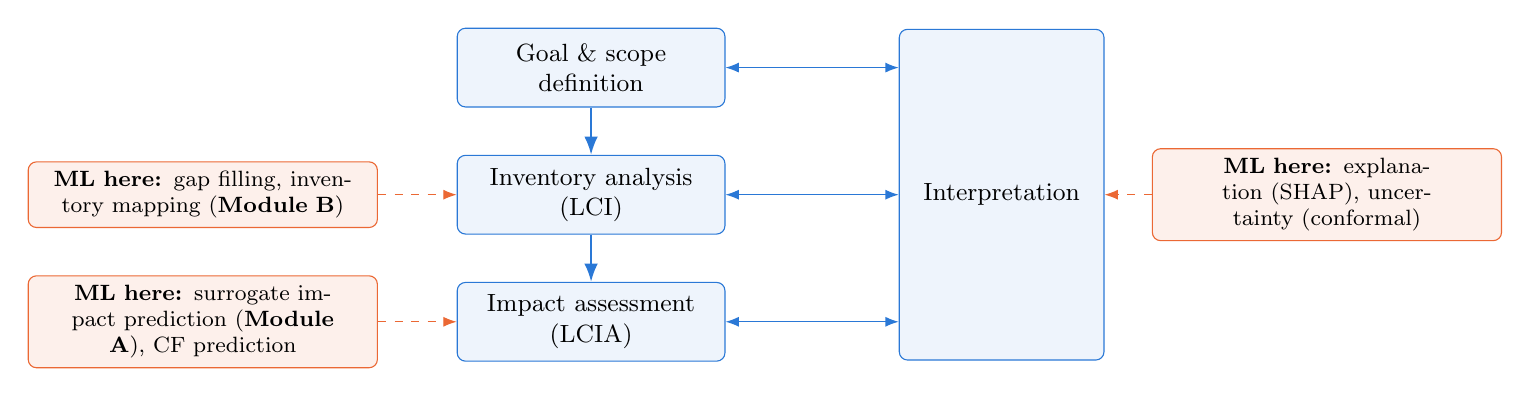
\begin{tikzpicture}[node distance=6mm and 10mm, every node/.style={font=\small},
  box/.style={draw=c1, fill=c1!8, rounded corners=3pt, minimum width=3.4cm, minimum height=1cm, align=center},
  ml/.style={draw=c2, fill=c2!10, rounded corners=3pt, align=center, font=\footnotesize, text width=4.2cm}]
\node[box] (g) {Goal \& scope\\definition};
\node[box, below=of g] (i) {Inventory analysis\\(LCI)};
\node[box, below=of i] (a) {Impact assessment\\(LCIA)};
\node[box, right=22mm of i, minimum height=4.2cm, minimum width=2.6cm] (int) {Interpretation};
\draw[-{Latex}, thick, c1] (g) -- (i); \draw[-{Latex}, thick, c1] (i) -- (a);
\foreach \n in {g,i,a} \draw[{Latex}-{Latex}, c1] (\n.east) -- (\n.east -| int.west);
\node[ml, left=10mm of i] (m1) {\textbf{ML here:} gap filling, inventory mapping (\textbf{Module B})};
\node[ml, left=10mm of a] (m2) {\textbf{ML here:} surrogate impact prediction (\textbf{Module A}), CF prediction};
\node[ml, right=6mm of int] (m3) {\textbf{ML here:} explanation (SHAP), uncertainty (conformal)};
\draw[-{Latex}, dashed, c2] (m1) -- (i); \draw[-{Latex}, dashed, c2] (m2) -- (a); \draw[-{Latex}, dashed, c2] (m3) -- (int);
\end{tikzpicture}}
\caption{The four ISO 14040/44 phases of LCA and where AI/ML methods integrate (dashed). Bold labels mark the parts implemented in this thesis.}
\label{fig:lca-phases}
\end{figure}

\subsection{Impact categories and the EF 3.0 method}

Results in this thesis use the European Commission's Environmental Footprint (EF~3.0) LCIA method
\citep{fazio2018}, which reports 16 midpoint indicators -- climate change, ozone depletion,
ionising radiation, photochemical ozone formation, particulate matter, human toxicity (cancer and
non-cancer), acidification, eutrophication (freshwater, marine, terrestrial), freshwater
ecotoxicity, land use, and depletion of water, fossil and mineral resources -- and a weighted
\emph{single score} in milli-points (mPt). Many of these indicators are strongly correlated across
products \citep{steinmann2016}, which suggests that a model which learns one indicator well may
transfer to others; this is tested in Section~\ref{sec:e3}.

\subsection{Types of LCA data}

\begin{itemize}
  \item \textbf{Process-based LCI databases} (e.g.\ ecoinvent \citep{wernet2016}, AGRIBALYSE
  \citep{agribalyse2020}) model individual unit processes in physical units; accurate but costly
  and (in ecoinvent's case) licensed.
  \item \textbf{Environmentally extended input--output (EEIO) models} (e.g.\ USEEIO
  \citep{yang2017useeio}) give impacts per unit of monetary spend by economic sector; complete
  coverage but coarse resolution.
  \item \textbf{Product-level result databases} such as the AGRIBALYSE synthesis tables give
  ready-computed impacts for finished products, which is precisely the supervised-learning target
  needed here.
\end{itemize}

\subsection{Why LCA is slow: the data bottleneck}

Reap et al.\ \citep{reap2008} identified data availability and quality as a central unresolved
problem in LCA, and Hellweg and Milà~i~Canals \citep{hellweg2014} highlight the need for faster,
streamlined approaches that keep scientific robustness. Two specific symptoms motivate this work:
(i) \emph{missing data} for new or niche products, and (ii) the \emph{mapping effort} needed to
connect product descriptions to database processes.

\section{AI/ML in LCA: a structured review}

Ghoroghi et al.\ \citep{ghoroghi2022} systematically reviewed ML applications in LCA and found
them concentrated in optimisation, prediction of impacts, and support for inventory compilation,
while noting gaps in transparency, uncertainty treatment and generalisability. Algren et al.\
\citep{algren2021} similarly survey ML methods for handling incomplete or uncertain LCA data.
The literature can be organised by the LCA phase that ML supports (Table~\ref{tab:lit}).

\subsection{Inventory gap filling}

Hou et al.\ \citep{hou2018} estimated missing unit-process flows in ecoinvent with a
similarity-based approach, accurate when fewer than about 5\% of flows are missing. Zhao et al.\
\citep{zhao2021} extended this with decision trees, classifying zero/non-zero flows and estimating
non-zero values with $R^2>0.7$ when under 20\% of a process is missing. These works operate on the
inventory matrix itself and require licensed process data.

\subsection{Surrogate models for rapid impact screening}

Song, Keller and Suh \citep{song2017} trained neural networks on molecular descriptors to predict
the cradle-to-gate impacts of chemicals, reaching $R^2$ of 0.87 for the Eco-indicator 99 score but
only 0.48 for global warming, and stressed that \emph{applicability domains} matter when
interpreting such screening predictions. This is the closest conceptual precedent for Module~A:
learn a direct map from cheap descriptors to impacts. In the food domain, Clark et al.\
\citep{clark2022} estimated four environmental indicators for 57{,}000 UK and Irish products by
inferring ingredient composition from ingredient lists and pairing it with LCA data -- a
rule-based rather than learned approach, but one that shows the value of ingredient information.

\subsection{NLP for mapping products to LCA data}

Balaji et al.\ \citep{balaji2023caml} (CaML) used pre-trained sentence-transformer embeddings
\citep{reimers2019} to map product descriptions to EEIO industry sectors in a zero-shot manner,
ranking the top-5 candidates for human confirmation and reporting a mean absolute percentage error
of about 22\% without domain labels. This motivates Module~B, which maps to \emph{product-level
process datasets} instead of sectors, compares several encoders, and tests a cross-lingual setting.

\subsection{Explainability and uncertainty}

Tree ensembles such as Random Forests \citep{breiman2001} and gradient boosting (XGBoost
\citep{chen2016xgboost}) are strong on tabular data, and SHAP values \citep{lundberg2017,lundberg2020}
provide additive, locally exact explanations for them. For uncertainty, conformal prediction
\citep{vovk2005,lei2018,angelopoulos2023} yields prediction intervals with finite-sample coverage
guarantees that do not depend on the model being correct -- an attractive property for LCA, where
uncertainty reporting is required by ISO~14044 but is rarely provided by ML surrogates.

\begin{table}[ht]
\centering\small
\caption{Representative AI/ML-in-LCA studies and how this thesis relates to them.}
\label{tab:lit}
\begin{tabularx}{\textwidth}{@{}p{2.6cm}p{2.4cm}Xp{2.3cm}@{}}
\toprule
Study & LCA phase & Approach & Gap addressed here \\
\midrule
Hou et al.\ 2018 \citep{hou2018} & Inventory & Similarity-based estimation of missing flows (ecoinvent) & Open data; product level \\
Zhao et al.\ 2021 \citep{zhao2021} & Inventory & Decision trees for missing flows & Uncertainty intervals \\
Song et al.\ 2017 \citep{song2017} & Impact & ANN from molecular descriptors to impacts & Explainability; unseen-category test \\
Clark et al.\ 2022 \citep{clark2022} & Inventory/Impact & Ingredient-list inference for 57k foods & Learned model; uncertainty \\
Balaji et al.\ 2023 \citep{balaji2023caml} & Inventory mapping & Zero-shot sentence similarity to EEIO sectors & Process-level, multilingual, encoder benchmark \\
Ghoroghi et al.\ 2022 \citep{ghoroghi2022} & Review & Survey of ML in LCA & -- \\
\midrule
\textbf{This thesis} & Mapping + Impact + Interpretation & XGBoost surrogate + E5 mapping + SHAP + conformal, integrated tool & -- \\
\bottomrule
\end{tabularx}
\end{table}

\section{Research gap}

From the review, four gaps emerge that this thesis addresses together:
\begin{enumerate}
  \item \textbf{Evaluation realism.} Most surrogate studies report random-split accuracy, which
  rewards memorising near-duplicates. Performance on genuinely new categories is rarely reported.
  \item \textbf{Uncertainty.} ML predictions in LCA are usually point estimates without calibrated
  intervals.
  \item \textbf{Transparency.} Black-box predictions are hard for LCA practitioners to trust or audit.
  \item \textbf{Integration.} Estimation and mapping are studied separately, though in practice
  they form one workflow (describe $\rightarrow$ map $\rightarrow$ estimate $\rightarrow$
  interpret).
\end{enumerate}

\chapter{Data}
\label{ch:data}

\section{Choice of database}

A central constraint of this work was to use only data that are \emph{openly licensed,
downloadable and verifiable} by any examiner. Commercial process databases (e.g.\ ecoinvent) were
therefore excluded. AGRIBALYSE (ADEME and INRAE, France) \citep{agribalyse2020,agribalyse31} was
selected because it is (i) published under the French open licence (Licence Ouverte/Etalab);
(ii) product-level, i.e.\ it reports finished-food impacts that can serve directly as
supervised-learning targets; (iii) computed with one consistent method (EF~3.0) and system
boundary; and (iv) accompanied by recipe and life-cycle-stage breakdowns.

\section{Source files}

Three CSV tables of AGRIBALYSE~3.1 were downloaded from the ADEME open-data portal (via
\texttt{data.gouv.fr}) on 5~November~2026:

\begin{table}[ht]
\centering\small
\caption{AGRIBALYSE 3.1 tables used.}
\label{tab:files}
\begin{tabularx}{\textwidth}{@{}lrrX@{}}
\toprule
Table & Rows & Columns & Content and use \\
\midrule
Synthèse (synthesis) & 2{,}451 & 32 & One row per product: names (FR/EN), food group and sub-group,
delivery mode, packaging data source, consumer preparation, season and air-freight flags, Data
Quality Rating (DQR), 16 EF~3.0 indicators + single score. \textbf{Targets and main features.} \\
Détail par ingrédient & 8{,}882 & 24 & Recipe ingredients of composite products. \textbf{Only the
\emph{presence} of each ingredient is used} (its impact columns are never used). \\
Détail par étape & 2{,}451 & 131 & Impacts split by life-cycle stage. \textbf{Descriptive analysis
only}, never a model input. \\
\bottomrule
\end{tabularx}
\end{table}

\section{Cleaning}

\begin{itemize}
  \item The synthesis file contains $\sim$12{,}500 empty trailing rows; these were dropped,
        leaving exactly 2{,}451 products with complete impact values.
  \item Category labels were stripped of whitespace (e.g.\ \texttt{"Four "} vs \texttt{"Four"})
        and translated to English for presentation; the 61 sub-group labels have an
        English display map.
  \item The French category \emph{``Pas de préparation''} is stored as \texttt{No preparation};
        storing it as \texttt{None} would be silently parsed as missing by \texttt{pandas}.
  \item In the ingredient table the pseudo-ingredient \emph{``Autres étapes''} (other steps) was
        removed, giving 5{,}062 product--ingredient links over 286 distinct ingredients and
        1{,}094 composite products.
  \item For log-scale modelling of other impact categories, products with non-positive values
        were excluded for that indicator only: 34 for land use (soil-carbon credits) and 1 for
        water use.
\end{itemize}

\section{The no-leakage rule}

The stage table and the per-ingredient impacts \emph{add up to} the target. A model given these
would trivially reproduce the answer and would be useless in practice, because an analyst who
already has them has already done the LCA. All features were therefore restricted to information
available \emph{before} an LCA: product name, category, storage/delivery mode, consumer
preparation, packaging data source, season and air-freight flags, and the list (not the masses) of
recipe ingredients.

\section{Exploratory analysis}

\subsection{Distribution of the target}

Climate-change impact ranges from 0.0003~kg~\co/kg (tap water) to 52.5~kg~\co/kg (lamb), with
median 2.78 and mean 5.76: the distribution is strongly right-skewed and spans five orders of
magnitude (Figure~\ref{fig:dist}, Table~\ref{tab:groups}). All models are therefore trained on
$y = \log_{10}(\text{GWP})$, which turns multiplicative errors into additive ones and prevents a few
high-impact meats from dominating the loss.

\begin{figure}[ht]
\centering
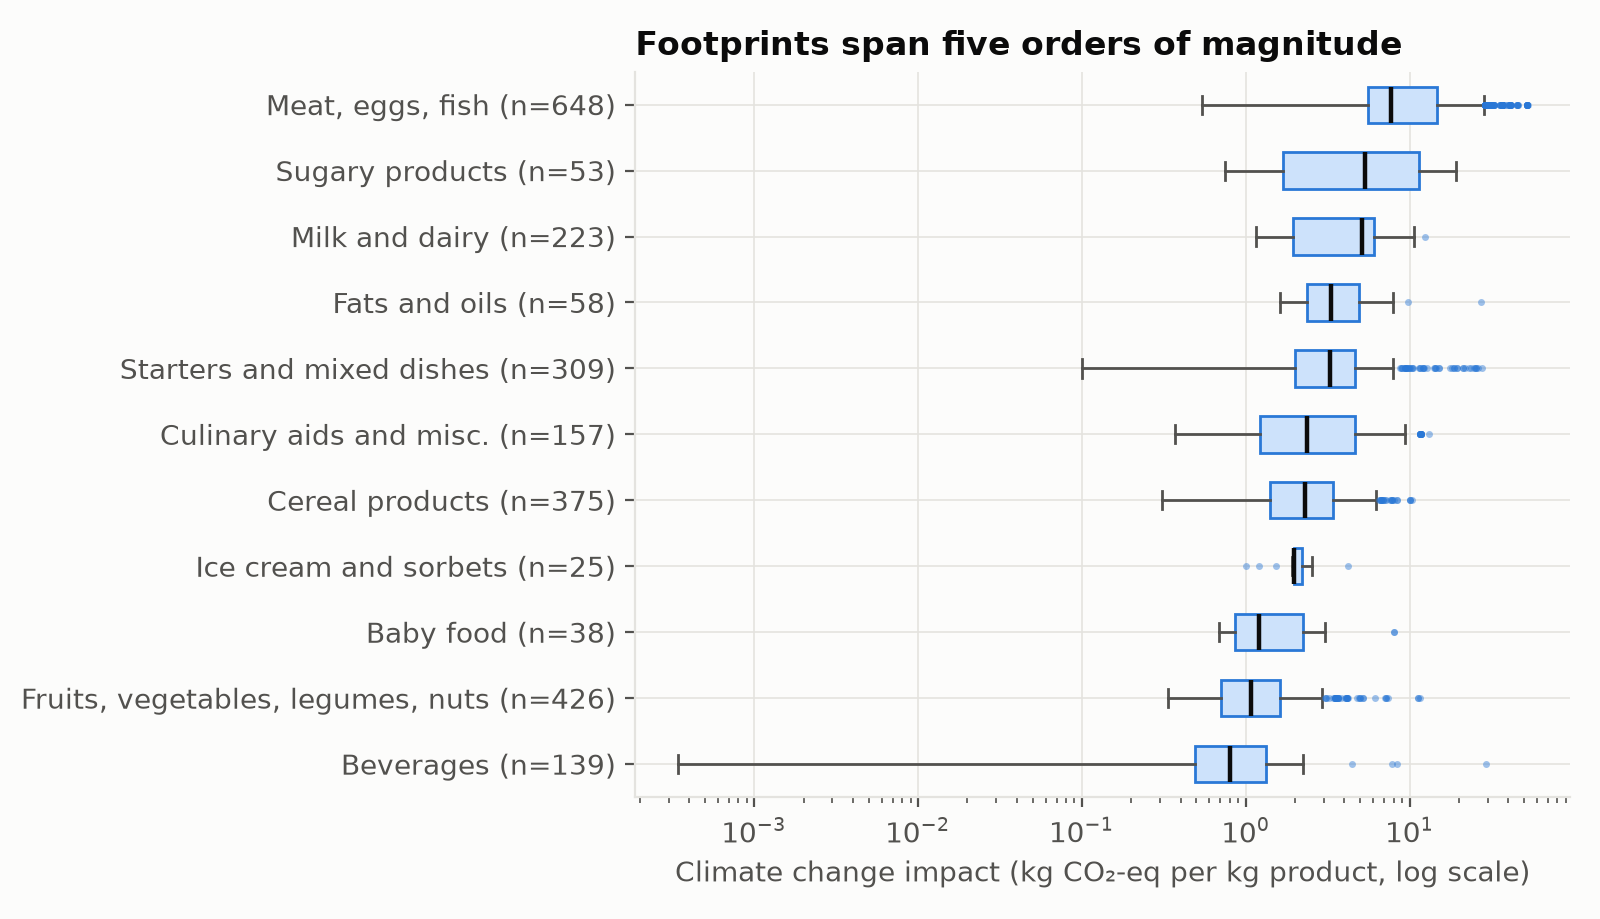
\includegraphics[width=\textwidth]{f1_gwp_by_group}
\caption{Climate-change impact per kg by food group (log scale). Boxes show the inter-quartile range; dots are individual products.}
\label{fig:dist}
\end{figure}

\begin{table}[ht]
\centering\small
\caption{Products and climate impact (kg \co/kg) by food group.}
\label{tab:groups}
\begin{tabular}{@{}lrrrrr@{}}
\toprule
Food group & $n$ & Median & Min & Max & Composite (\%) \\
\midrule
Meat, eggs, fish & 648 & 7.75 & 0.54 & 52.50 & 19 \\
Fruits, vegetables, legumes, nuts & 426 & 1.08 & 0.33 & 11.60 & 12 \\
Cereal products & 375 & 2.30 & 0.31 & 10.30 & 81 \\
Starters and mixed dishes & 309 & 3.26 & 0.10 & 27.80 & 92 \\
Milk and dairy & 223 & 5.16 & 1.15 & 12.50 & 31 \\
Culinary aids and misc. & 157 & 2.37 & 0.37 & 13.20 & 48 \\
Beverages & 139 & 0.80 & 0.0003 & 29.10 & 47 \\
Fats and oils & 58 & 3.30 & 1.63 & 27.40 & 28 \\
Sugary products & 53 & 5.32 & 0.75 & 19.30 & 87 \\
Baby food & 38 & 1.21 & 0.68 & 8.05 & 100 \\
Ice cream and sorbets & 25 & 1.98 & 1.00 & 4.24 & 100 \\
\midrule
\textbf{All} & \textbf{2,451} & \textbf{2.78} & \textbf{0.0003} & \textbf{52.50} & \textbf{45} \\
\bottomrule
\end{tabular}
\end{table}

Two observations matter for modelling. First, \emph{between-group} differences are large (median
meat footprint is seven times that of fruit and vegetables), so category information alone is
valuable. Second, \emph{within-group} spread is also large (a factor of 100 within meat), so
category averages are insufficient -- finer product information is required.

\subsection{Where in the life cycle do impacts arise?}

Figure~\ref{fig:stages} aggregates the stage table by food group. Agriculture dominates for
animal products (88\% for meat, eggs and fish; 79\% for dairy), while packaging and transport
become significant for beverages and fruit and vegetables. Since agricultural impact is driven
mainly by \emph{what} the food is (species, crop), this suggests that product identity --
captured by its name and ingredients -- should be the most informative feature, which is
confirmed in Section~\ref{sec:ablation}.

\begin{figure}[ht]
\centering
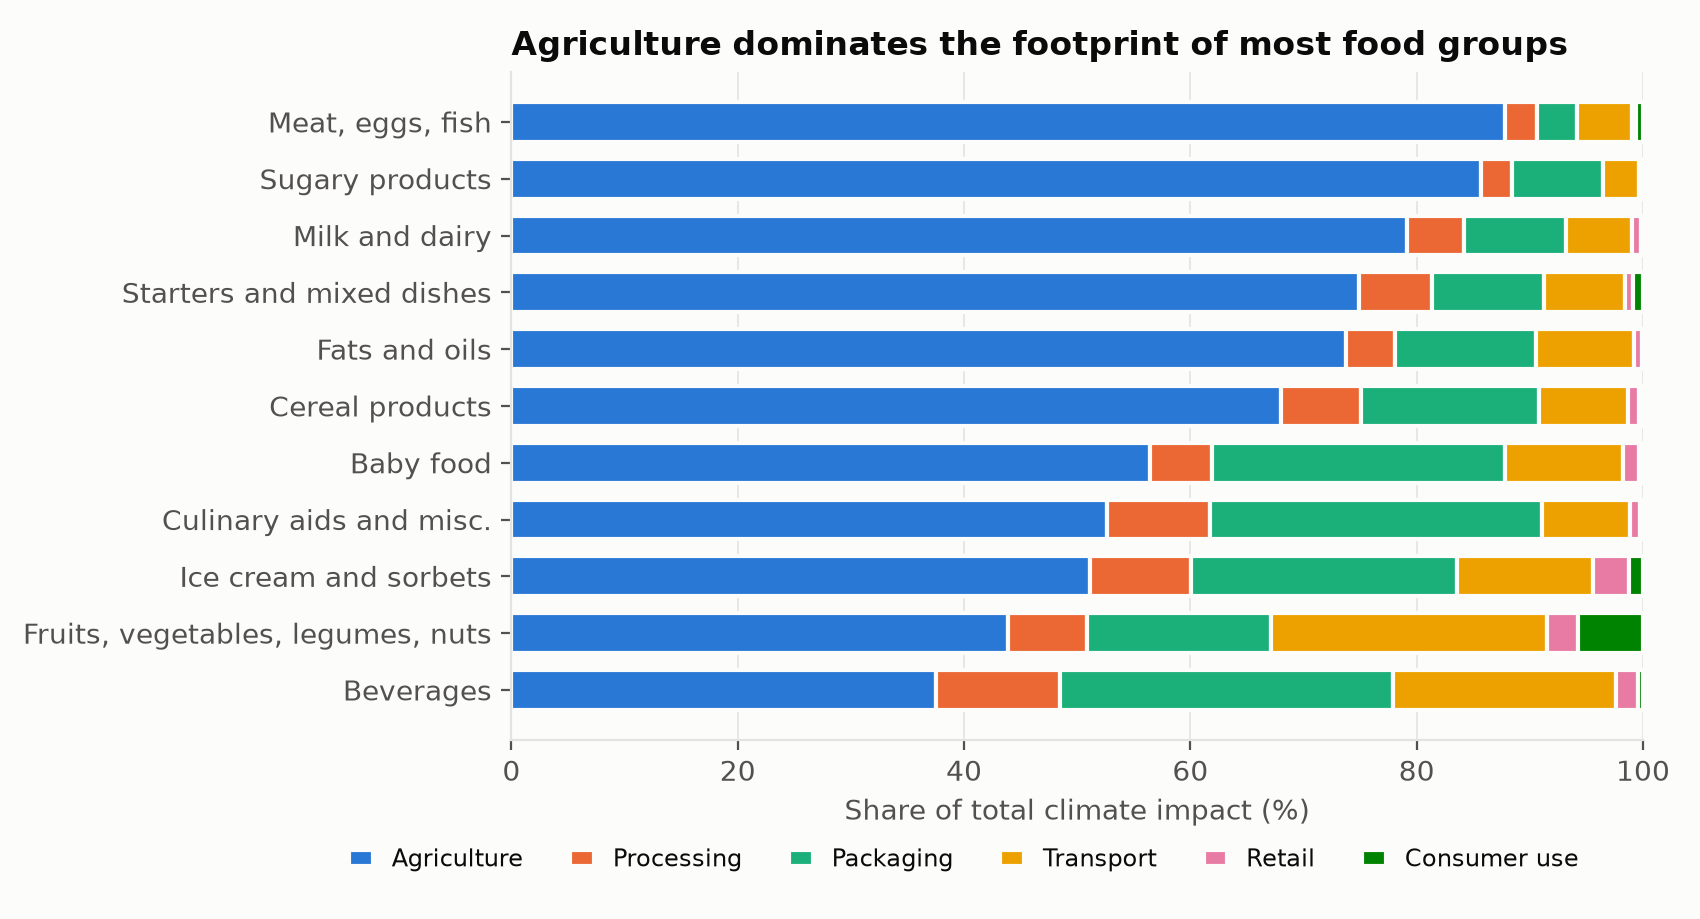
\includegraphics[width=\textwidth]{f2_stage_contribution}
\caption{Share of climate impact by life-cycle stage and food group (descriptive only; never a model input).}
\label{fig:stages}
\end{figure}

\subsection{Categorical descriptors}

Delivery mode: chilled 1{,}223, ambient long shelf-life 821, ambient medium 238, frozen 97,
ambient short 72. Consumer preparation: none 1{,}646, oven 300, microwave 262, boiling 119,
pan-frying 72, refrigerated at home 52. Packaging data come from AGRIBALYSE-specific data for
1{,}284 products and from proxies for 1{,}167. The mean Data Quality Rating is 2.46
(1 = best, 5 = worst), indicating generally good but heterogeneous underlying data quality.
Season and air-freight flags are almost constant (only 4 and 2 exceptions), so they carry little
information.

\chapter{Methodology}
\label{ch:method}

\section{Overall framework}

Figure~\ref{fig:arch} shows the integrated workflow. A user describes a product in free text.
Module~B retrieves the most similar LCA datasets and pre-fills the product's attributes, which the
user may correct. Module~A then predicts the impact, attaches a calibrated interval and explains the
prediction. An applicability-domain check warns when the description is unlike anything in the
database.

\begin{figure}[ht]
\centering
\resizebox{\textwidth}{!}{%
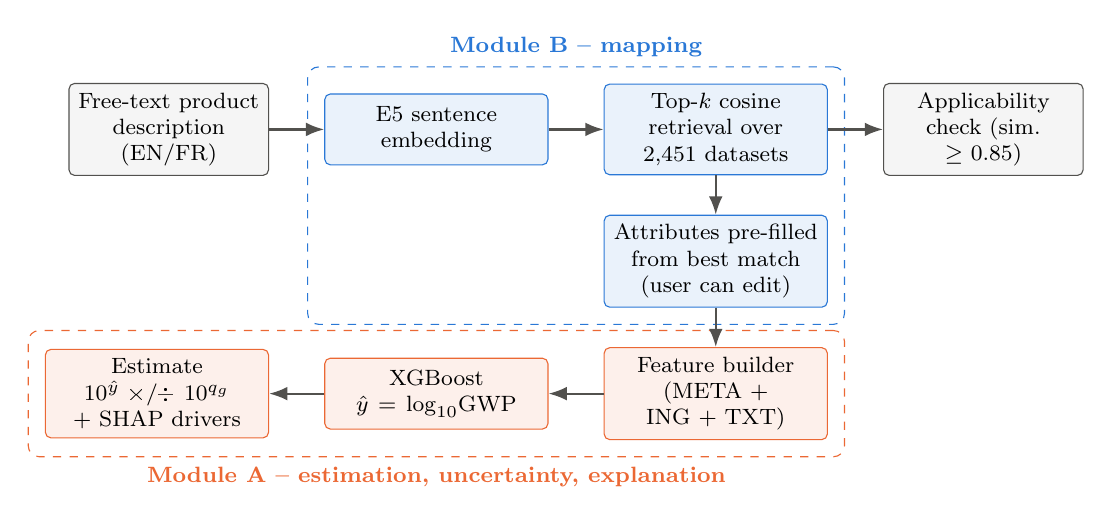
\begin{tikzpicture}[node distance=5mm and 7mm, every node/.style={font=\footnotesize},
  io/.style={draw=inkgray, fill=gray!8, rounded corners=2pt, align=center, minimum height=9mm, text width=2.3cm},
  mb/.style={draw=c1, fill=c1!10, rounded corners=2pt, align=center, minimum height=9mm, text width=2.6cm},
  ma/.style={draw=c2, fill=c2!10, rounded corners=2pt, align=center, minimum height=9mm, text width=2.6cm},
  arr/.style={-{Latex}, thick, inkgray}]
\node[io] (in) {Free-text product\\description (EN/FR)};
\node[mb, right=of in] (emb) {E5 sentence\\embedding};
\node[mb, right=of emb] (ret) {Top-$k$ cosine\\retrieval over\\2,451 datasets};
\node[io, right=of ret] (ad) {Applicability\\check (sim.\ $\geq$ 0.85)};
\node[mb, below=of ret] (attr) {Attributes pre-filled\\from best match\\(user can edit)};
\node[ma, below=of attr] (fe) {Feature builder\\(META + ING + TXT)};
\node[ma, left=of fe] (xgb) {XGBoost\\$\hat y=\log_{10}$GWP};
\node[ma, left=of xgb] (out) {Estimate\\$10^{\hat y}$ ×/÷ $10^{q_g}$\\+ SHAP drivers};
\draw[arr] (in) -- (emb); \draw[arr] (emb) -- (ret); \draw[arr] (ret) -- (ad);
\draw[arr] (ret) -- (attr); \draw[arr] (attr) -- (fe); \draw[arr] (fe) -- (xgb); \draw[arr] (xgb) -- (out);
\begin{scope}[on background layer]
\node[draw=c1, dashed, rounded corners, fit=(emb)(ret)(attr), inner sep=6pt, label={[c1,font=\footnotesize\bfseries]above:Module B -- mapping}] {};
\node[draw=c2, dashed, rounded corners, fit=(fe)(xgb)(out), inner sep=6pt, label={[c2,font=\footnotesize\bfseries]below:Module A -- estimation, uncertainty, explanation}] {};
\end{scope}
\end{tikzpicture}}
\caption{Integrated screening framework. Module B (blue) maps text to datasets; Module A (orange) estimates, quantifies uncertainty and explains.}
\label{fig:arch}
\end{figure}

\section{Problem formulation (Module A)}

For product $i$ with pre-LCA descriptor vector $\mathbf{x}_i$ and impact $I_i>0$, learn
\[
  \hat f:\ \mathbf{x}\ \mapsto\ \hat y = \log_{10}\hat I, \qquad
  \hat f = \arg\min_f \sum_i \big(y_i - f(\mathbf{x}_i)\big)^2 + \Omega(f),
\]
where $y_i=\log_{10} I_i$ and $\Omega$ is a complexity penalty. Squared error on the log scale
corresponds to penalising the \emph{ratio} $\hat I / I$, which matches how LCA practitioners think
about screening accuracy (``within a factor of two'').

\section{Feature engineering}

Features are built in four blocks, used incrementally in the ablation study:

\begin{description}
  \item[META] One-hot encodings of food group (11 levels), sub-group (61), delivery mode (5),
  consumer preparation (6) and packaging data source (2); numeric season and air-freight codes;
  number of recipe ingredients and a composite-product flag.
  \item[ING] Binary indicators for each recipe ingredient occurring in at least five training
  products (125 ingredients); zero for non-composite products.
  \item[TXT] Binary bag-of-words from the English product name (words occurring in at least five
  training products, minus stop-words; 421 words), giving interpretable features such as \texttt{word:beef}.
  \item[KNN] (tested, not adopted) the similarity-weighted footprint of the $k=10$ most similar
  \emph{other} training products in the E5 embedding space, with softmax weights
  $w_j \propto \exp(s_j/T)$, $T=0.01$.
\end{description}

All vocabularies (category levels, ingredients, words) are fitted on the training fold only. The
final model has 635 features.

\section{Models}

\begin{enumerate}
  \item \textbf{Global median} -- predicts the training median for every product (lower bound).
  \item \textbf{Sub-group median (proxy)} -- predicts the median of the product's sub-group
  (falling back to its group, then globally). This mimics the common practitioner shortcut of
  using a category-average emission factor, and is the main baseline to beat.
  \item \textbf{Ridge regression} \citep{hoerl1970} -- linear model with $L_2$ penalty ($\alpha=3$).
  \item \textbf{Random Forest} \citep{breiman2001} -- 500 trees, min.\ leaf size 2, 30\% of
  features per split.
  \item \textbf{XGBoost} \citep{chen2016xgboost} -- gradient-boosted trees (600 trees, learning
  rate 0.03, max depth 6, row subsample 0.8, column subsample 0.5, min child weight 2,
  $\lambda=1$). Hyper-parameters are standard values for small tabular datasets and were fixed
  \emph{a priori}, not tuned on the test folds.
  \item \textbf{kNN on text embedding} -- Module B used directly as a regressor (KNN block alone).
  \item \textbf{XGBoost + kNN} -- XGBoost with the KNN block stacked as an extra feature; the kNN
  value for training rows is computed leave-one-out so it never sees the row's own target.
\end{enumerate}

\section{Validation design}
\label{sec:validation}

Two 5-fold cross-validation schemes answer two different practical questions:

\begin{description}
  \item[Random CV] Products are split at random. This answers: \emph{``How well does the model
  estimate a new product when similar products are already in the database?''} It is optimistic,
  because AGRIBALYSE contains near-duplicates (e.g.\ raw vs.\ cooked, oven vs.\ microwave
  variants of the same dish).
  \item[Leave-sub-group-out CV] \texttt{GroupKFold} by sub-group: every product of a sub-group is
  in the same fold, so test sub-groups are \emph{never seen} during training. This answers:
  \emph{``How well does the model generalise to a new kind of product?''} It is the honest lower
  bound.
\end{description}

All reported numbers are \emph{out-of-fold}: every product is predicted by a model that never saw it.

\section{Evaluation metrics}

With $y$ and $\hat y$ on the $\log_{10}$ scale and $I=10^y$:
\begin{itemize}
  \item $R^2$ on the log scale -- share of variance in $\log$ impact explained.
  \item Within-factor-2 rate $= \frac1n\sum_i \mathbf{1}\big[|y_i-\hat y_i|<\log_{10}2\big]$ --
  the most intuitive screening metric.
  \item Median absolute percentage error (MdAPE) and MAE in kg~\co/kg on the original scale.
  \item Spearman rank correlation -- whether the model ranks products correctly, which is what
  portfolio screening and hotspot prioritisation actually need.
\end{itemize}

\section{Uncertainty quantification: Mondrian split-conformal prediction}

Conformal prediction \citep{vovk2005,lei2018,angelopoulos2023} turns any point predictor into an
interval predictor with a distribution-free coverage guarantee. Given $n$ calibration residuals
$r_j=|y_j-\hat y_j|$ from data not used to fit the model, set
\[
  q = \text{Quantile}\Big(\{r_j\};\ \tfrac{\lceil (n+1)(1-\alpha)\rceil}{n}\Big), \qquad
  C(\mathbf{x}) = [\hat y - q,\ \hat y + q],
\]
which satisfies $\Pr(y\in C(\mathbf{x}))\ge 1-\alpha$ if calibration and test data are exchangeable.
On the original scale the interval is $\hat I \times\!/\!\div\, 10^{q}$.

Because prediction difficulty differs strongly between food groups (Figure~\ref{fig:dist}), a
\emph{Mondrian} (group-conditional) variant is used: a separate $q_g$ is computed for each food
group $g$ with at least 20 calibration products, with a global $q$ as fallback. This gives narrower
intervals for homogeneous groups and wider ones where data are heterogeneous, with approximately
group-wise coverage.

To evaluate coverage honestly, calibration is \emph{nested}: within each outer training fold, an
inner 5-fold CV produces out-of-fold residuals that define $q_g$; coverage and width are then
measured on the untouched outer test fold. The deployed model uses out-of-fold residuals from the
full dataset. Target miscoverage is $\alpha=0.10$.

\section{Explainability: SHAP}

For a tree ensemble $f$, the SHAP value $\phi_j(\mathbf{x})$ of feature $j$ is its Shapley value in
the cooperative game whose payoff is the model output \citep{lundberg2017}; the explanation is
additive,
\[
  f(\mathbf{x}) = \phi_0 + \sum_{j} \phi_j(\mathbf{x}),
\]
where $\phi_0$ is the mean prediction. TreeSHAP \citep{lundberg2020} computes these values exactly
and quickly. Because the target is $\log_{10}$ GWP, $10^{\phi_j}$ is the \emph{multiplicative
factor} by which feature $j$ moves the estimate, which is easy to communicate (``the word
\emph{lamb} multiplies the estimate by 2.4'').

\section{Module B: semantic mapping to LCA datasets}

\subsection{Encoders}

Each candidate encoder maps a text $t$ to a unit vector $\mathbf{e}(t)\in\mathbb{R}^d$; similarity
is the cosine $s(t,t')=\mathbf{e}(t)^\top\mathbf{e}(t')$, and retrieval returns the top-$k$ database
entries. Five encoders were compared:
\begin{itemize}
  \item TF-IDF over character 3--5-grams \citep{salton1988} (lexical baseline);
  \item paraphrase-multilingual-MiniLM-L12-v2 \citep{reimers2020};
  \item LaBSE \citep{feng2022labse};
  \item multilingual-E5-base and multilingual-E5-small \citep{wang2024e5}, using the
  recommended \texttt{query:}/\texttt{passage:} prefixes;
\end{itemize}
plus a hybrid (average of TF-IDF and E5-small similarities).

\subsection{Benchmark tasks}

Ground-truth mappings between external product lists and AGRIBALYSE do not exist publicly, so two
tasks with known correct answers were constructed from the database itself:
\begin{description}
  \item[T1 -- cross-lingual] query = French product name, corpus = 2{,}451 English LCI names.
  Simulates mapping a non-English bill of materials.
  \item[T2 -- terse query] query = first three words of the English name, corpus = full names.
  Simulates the short descriptions analysts actually type.
\end{description}
A retrieval is correct if the retrieved English name equals the true one (a strict criterion:
near-duplicate variants count as errors). Metrics are top-1 and top-5 accuracy, the share of
top-1 matches in the correct sub-group, and the share whose borrowed footprint lies within a factor
of two of the true value.

\subsection{Applicability domain}

For an out-of-scope description the nearest dataset is still returned, so a similarity threshold
is needed. It was calibrated on two probe sets (\texttt{src/ood\_threshold.py}): the 2{,}451
in-domain terse queries of task T2, and 20 deliberately out-of-domain queries -- non-food goods
(e.g.\ ``car tyre'', ``laptop'', ``cement bag'') and Indian foods absent from AGRIBALYSE
(``paneer'', ``idli'', ``dhokla''). With E5-small, the highest out-of-domain similarity was 0.848
(``petrol''), while the 1st percentile of in-domain similarities was 0.873. A threshold of
$s<0.85$ therefore flags all 20 out-of-domain probes and only 0.04\% (1 of 2{,}451) of in-domain
queries, and triggers the warning in the tool. Cross-lingual queries score systematically lower
(e.g.\ the French ``yaourt nature'' is matched correctly at 0.81), so the warning advises
non-English users to rephrase in English.

\section{Implementation}

The pipeline is implemented in Python~3.12 with pandas, scikit-learn \citep{pedregosa2011},
XGBoost~3.2, SHAP, Sentence-Transformers and Streamlit. All randomness is seeded (seed 42); the
complete pipeline runs in about 15 minutes on a laptop CPU, and every table and figure in this
thesis is regenerated by six scripts (Appendix~\ref{app:repro}).

\chapter{Results}
\label{ch:results}

Five experiments were run. Unless stated otherwise the target is climate change (kg~\co/kg),
modelled as $\log_{10}$, and all numbers are out-of-fold over 5 folds (seed 42).

\section{E1 -- Model comparison}
\label{sec:e1}

\begin{table}[ht]
\centering\small
\caption{Model comparison for climate change under the two validation schemes. Best ML values in bold; ``proxy'' is the practitioner baseline.}
\label{tab:e1}
\begin{tabular}{@{}lrrrrrr@{}}
\toprule
& \multicolumn{3}{c}{Random 5-fold CV} & \multicolumn{3}{c}{Leave-sub-group-out CV} \\
\cmidrule(lr){2-4}\cmidrule(l){5-7}
Method & $R^2_{\log}$ & ${<}2\times$ (\%) & Spearman & $R^2_{\log}$ & ${<}2\times$ (\%) & Spearman \\
\midrule
Global median & $-0.01$ & 44.0 & $-0.02$ & $-0.03$ & 42.2 & $-0.20$ \\
Sub-group median (proxy) & 0.62 & 77.4 & 0.82 & 0.33 & 54.2 & 0.58 \\
Ridge & 0.81 & 89.2 & 0.91 & 0.57 & 69.0 & 0.77 \\
Random Forest & 0.83 & 91.0 & 0.92 & 0.58 & 69.9 & 0.77 \\
\textbf{XGBoost} & \textbf{0.84} & \textbf{91.1} & \textbf{0.92} & \textbf{0.62} & \textbf{72.4} & \textbf{0.78} \\
kNN on E5 embedding & 0.71 & 82.7 & 0.84 & 0.25 & 56.3 & 0.48 \\
XGBoost + kNN feature & 0.83 & 90.7 & 0.92 & 0.56 & 69.7 & 0.74 \\
\bottomrule
\end{tabular}
\end{table}

\begin{figure}[ht]
\centering
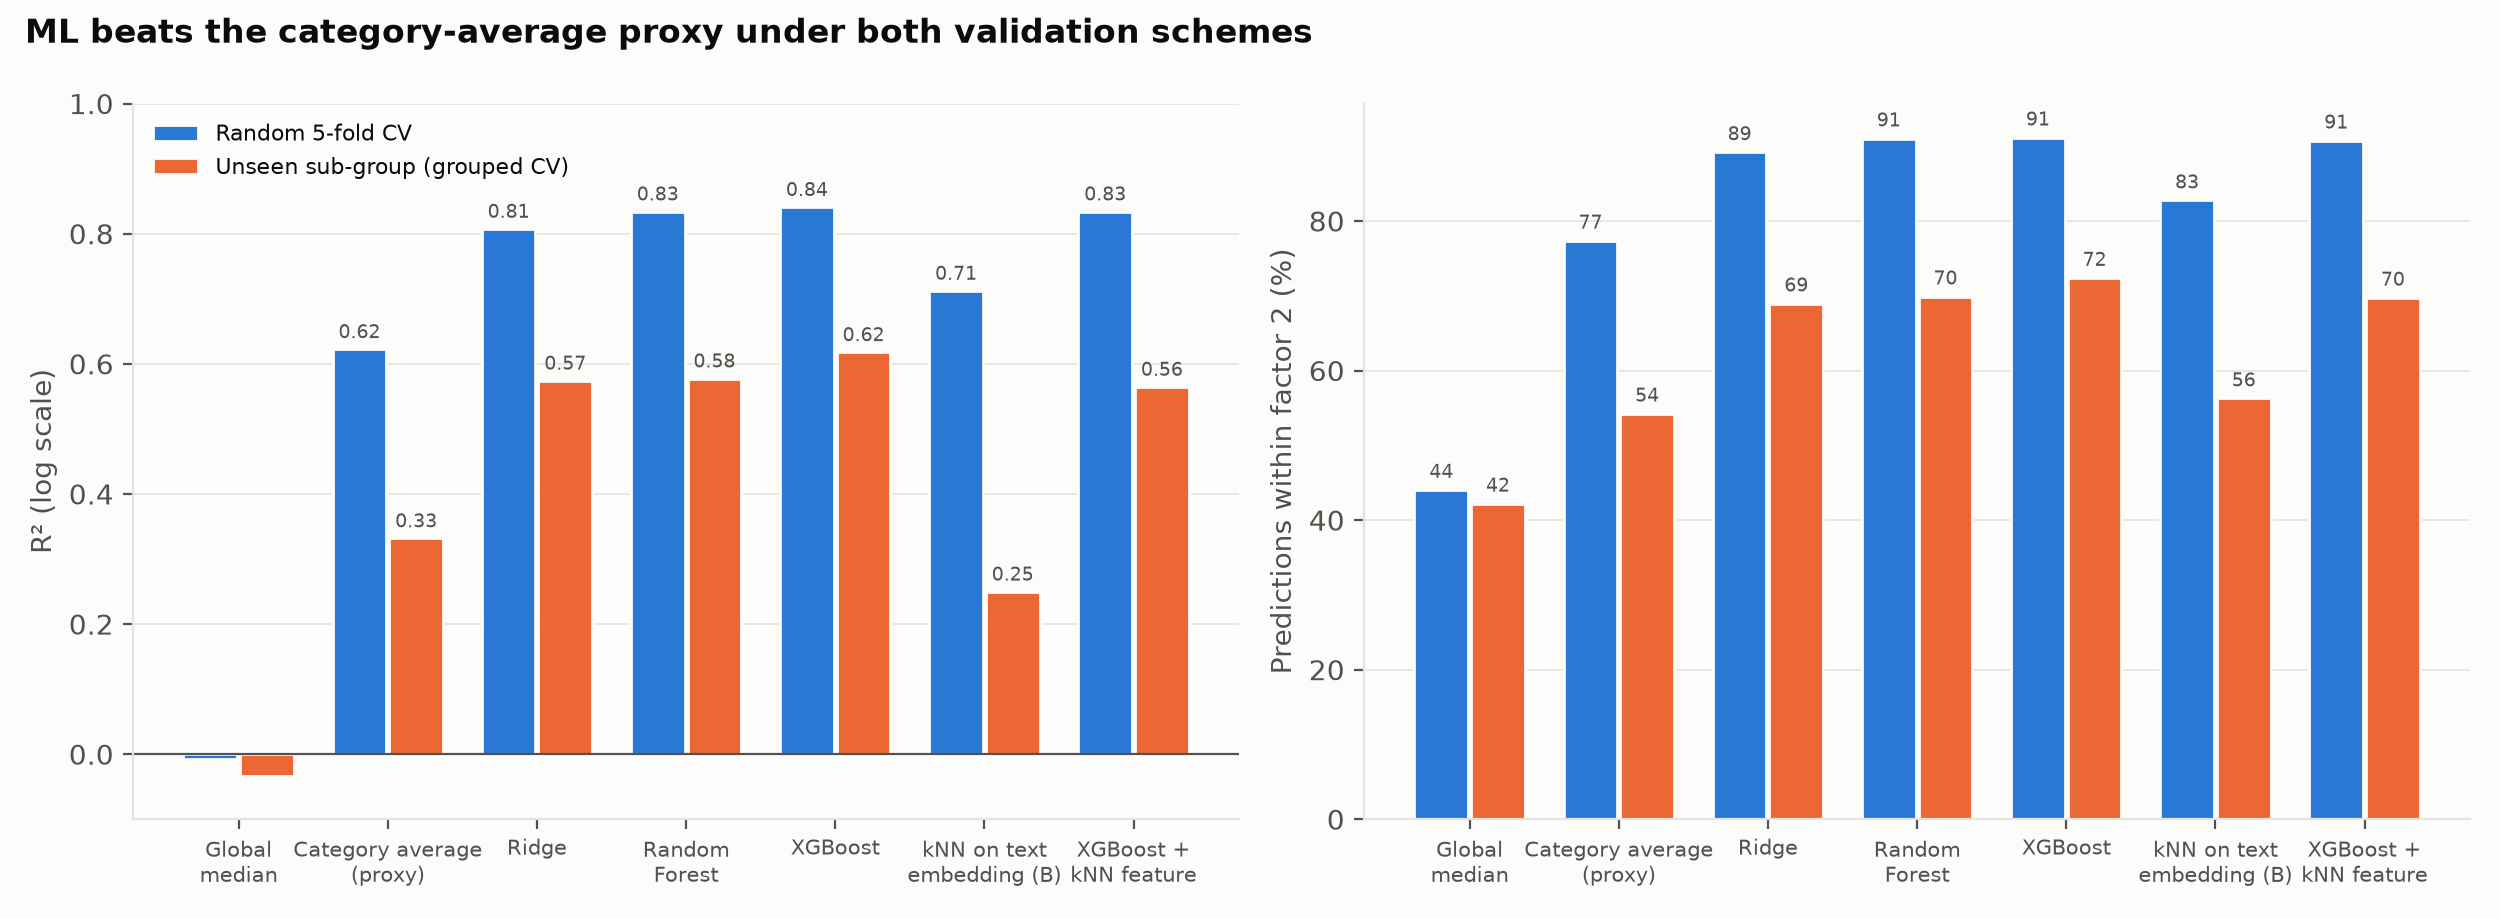
\includegraphics[width=\textwidth]{f3_model_comparison}
\caption{Model comparison: $R^2$ on the log scale (left) and share of predictions within a factor of two (right), for random and leave-sub-group-out CV.}
\label{fig:e1}
\end{figure}

Table~\ref{tab:e1} and Figure~\ref{fig:e1} answer \textbf{RQ1}. Under random CV, every ML model
clearly beats the category-average proxy; XGBoost raises $R^2_{\log}$ from 0.62 to 0.84 and the
within-factor-2 rate from 77\% to 91\%. Its median absolute percentage error is 19\% (proxy: 32\%)
and its MAE is 1.49~kg~\co/kg (proxy: 2.80). The Spearman correlation of 0.92 means that the
model ranks products almost correctly -- the property that matters most for screening.

The tree ensembles (Random Forest, XGBoost) outperform Ridge, indicating useful non-linear
interactions (e.g.\ the effect of ``chilled'' depends on the food group). XGBoost and Random
Forest are close; XGBoost is selected because it is best on the harder scheme.

\textbf{RQ2 -- generalisation.} When entire sub-groups are hidden, all methods degrade, as
expected. The proxy suffers most ($R^2$ 0.62 $\rightarrow$ 0.33): when a category is new, its
average is unknown and the method falls back to the group average. XGBoost retains $R^2=0.62$
and 72\% within a factor of two, because ingredient and name-word features transfer across
categories (e.g.\ \emph{beef} means high impact in any sub-group). The gap between the two schemes
(0.84 vs 0.62) is the honest measure of how much random CV benefits from near-duplicate products.

Figure~\ref{fig:pred} shows out-of-fold predictions against AGRIBALYSE values. Most points lie
within the factor-of-two band across four orders of magnitude. The largest errors are
instructive rather than random:
\begin{itemize}
  \item \textbf{Unique products} -- tap water (0.0003~kg~\co/kg) is predicted at 0.77 because
  nothing similar exists in the training data.
  \item \textbf{Air freight} -- mango pulp flown from Brazil (11.6, predicted 0.79) and French
  beans flown from Kenya (7.1, predicted 0.75). Only two products carry the air-freight flag, so
  the model cannot learn its effect; a rare but decisive life-cycle choice is invisible to a
  data-driven model.
  \item \textbf{High-impact tropical crops in low-impact groups} -- cocoa powder (29.1, predicted
  1.6), ground coffee (8.4, predicted 0.8) and cocoa butter sit in the beverage and fat groups,
  whose typical members have far lower footprints.
\end{itemize}
These failure modes point directly to the features a future version needs (transport mode,
origin, crop type), and they are discussed in Chapter~\ref{ch:discussion}.

\begin{figure}[ht]
\centering
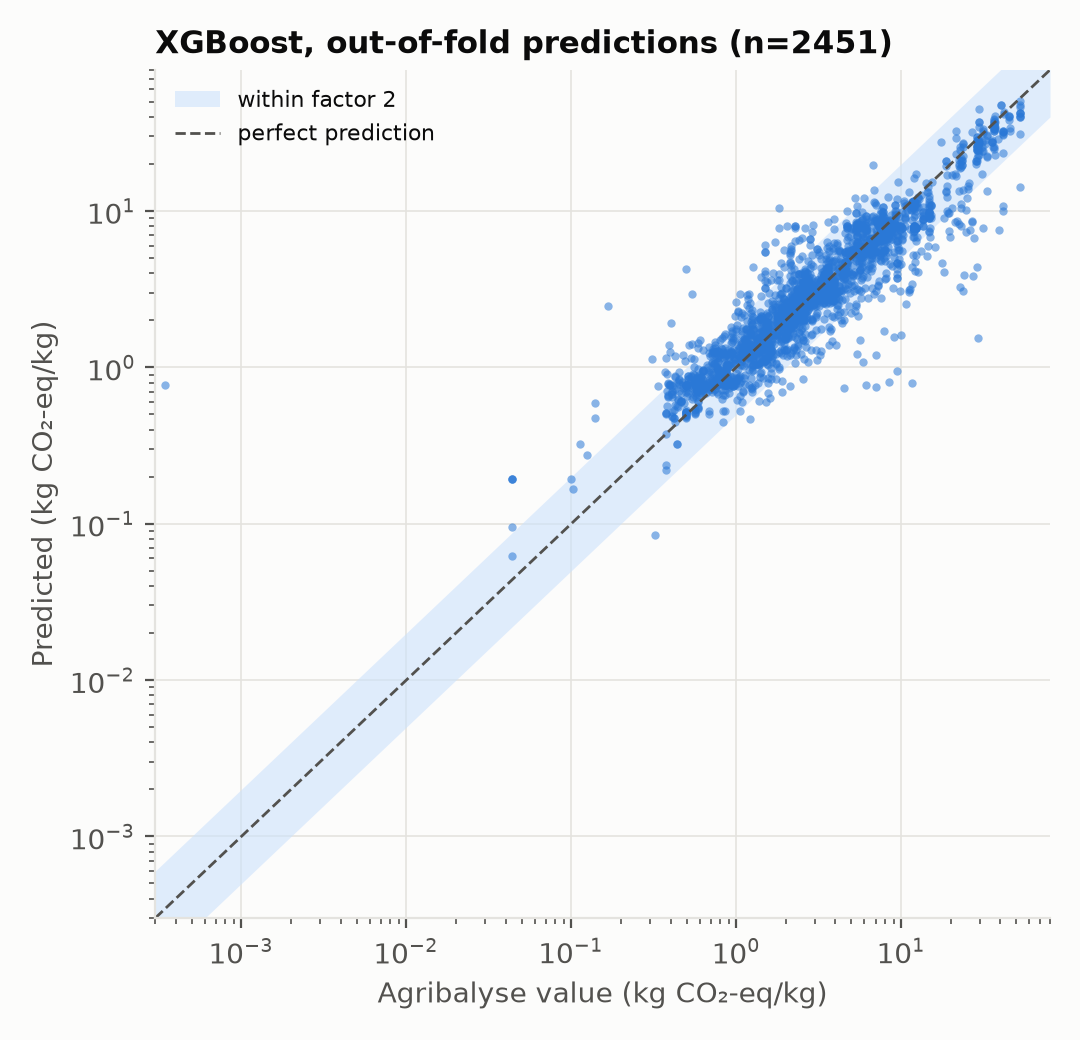
\includegraphics[width=0.62\textwidth]{f4_pred_vs_actual}
\caption{XGBoost out-of-fold predictions vs.\ AGRIBALYSE values (random CV, log--log). Shaded band: within a factor of two.}
\label{fig:pred}
\end{figure}

\section{E2 -- Feature ablation}
\label{sec:ablation}

\begin{table}[ht]
\centering\small
\caption{Feature ablation with XGBoost ($R^2_{\log}$ / within factor 2).}
\label{tab:e2}
\begin{tabular}{@{}lcc@{}}
\toprule
Feature set & Random CV & Leave-sub-group-out \\
\midrule
META (categories, storage, preparation, packaging) & 0.70 / 79.2\% & 0.48 / 64.0\% \\
+ ING (recipe ingredients) & 0.75 / 84.6\% & 0.52 / 67.2\% \\
+ TXT (product-name words) & \textbf{0.84 / 91.1\%} & \textbf{0.62 / 72.4\%} \\
+ KNN (E5-embedding neighbours) & 0.83 / 90.7\% & 0.56 / 69.7\% \\
\bottomrule
\end{tabular}
\end{table}

\begin{figure}[ht]
\centering
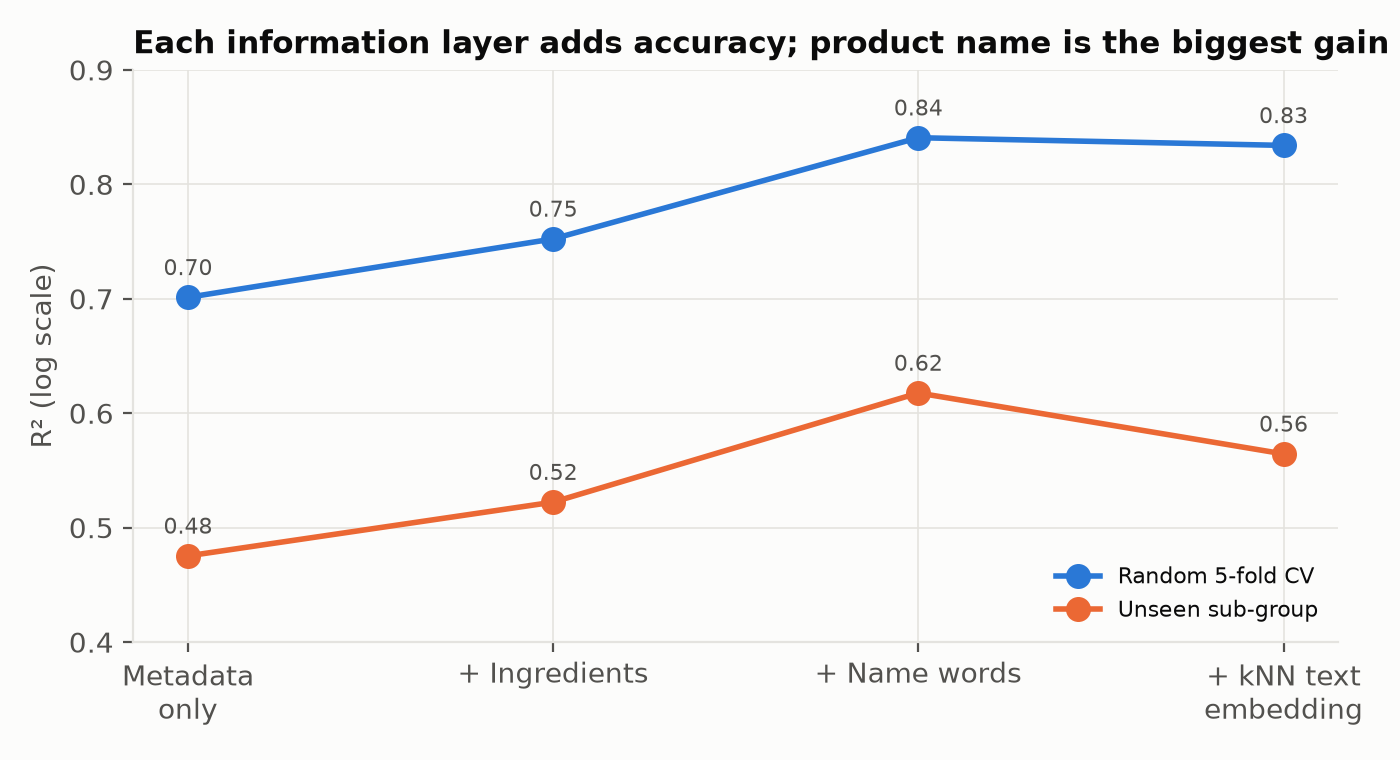
\includegraphics[width=0.8\textwidth]{f5_ablation}
\caption{Ablation: accuracy as information layers are added.}
\label{fig:ablation}
\end{figure}

Each pre-LCA information layer adds accuracy (Table~\ref{tab:e2}, Figure~\ref{fig:ablation}).
Metadata alone already beat the proxy (0.70 vs 0.62), ingredients add 0.05, and \textbf{product-name
words give the largest single gain} (+0.09 random, +0.10 unseen). This agrees with the stage
analysis in Chapter~\ref{ch:data}: impact is dominated by agriculture, i.e.\ by \emph{what} the
food is, which the name states directly (``lamb'', ``beef'', ``chocolate'').

A notable \emph{negative result} is that stacking the E5-embedding kNN estimate as a feature
did \emph{not} help; it slightly reduced accuracy, particularly on unseen sub-groups (0.62
$\rightarrow$ 0.56). The kNN estimate is largely redundant with the explicit word features, and on
new categories it imports the footprint of superficially similar but differently produced foods.
Embeddings were therefore kept for \emph{mapping} (Module B), where they excel (Section~\ref{sec:e5}),
and not used as a predictive feature.

\section{E3 -- Generalisation to other impact categories}
\label{sec:e3}

\begin{table}[ht]
\centering\small
\caption{Proxy vs.\ XGBoost for six EF 3.0 indicators (random CV).}
\label{tab:e3}
\begin{tabular}{@{}lrcccc@{}}
\toprule
& & \multicolumn{2}{c}{$R^2_{\log}$} & \multicolumn{2}{c}{Within $2\times$ (\%)} \\
\cmidrule(lr){3-4}\cmidrule(l){5-6}
Impact category (unit per kg) & $n$ & Proxy & XGBoost & Proxy & XGBoost \\
\midrule
Climate change (kg \co) & 2,451 & 0.62 & \textbf{0.84} & 77.4 & \textbf{91.1} \\
EF single score (mPt) & 2,451 & 0.64 & \textbf{0.84} & 78.2 & \textbf{90.4} \\
Land use (Pt) & 2,417 & 0.58 & \textbf{0.78} & 66.4 & \textbf{80.4} \\
Water use (m\textsuperscript{3} world-eq) & 2,450 & 0.27 & \textbf{0.64} & 64.8 & \textbf{80.5} \\
Marine eutrophication (kg N-eq) & 2,451 & 0.59 & \textbf{0.78} & 69.4 & \textbf{83.5} \\
Particulate matter (disease inc.) & 2,451 & 0.70 & \textbf{0.86} & 73.2 & \textbf{85.8} \\
\bottomrule
\end{tabular}
\end{table}

\begin{figure}[ht]
\centering
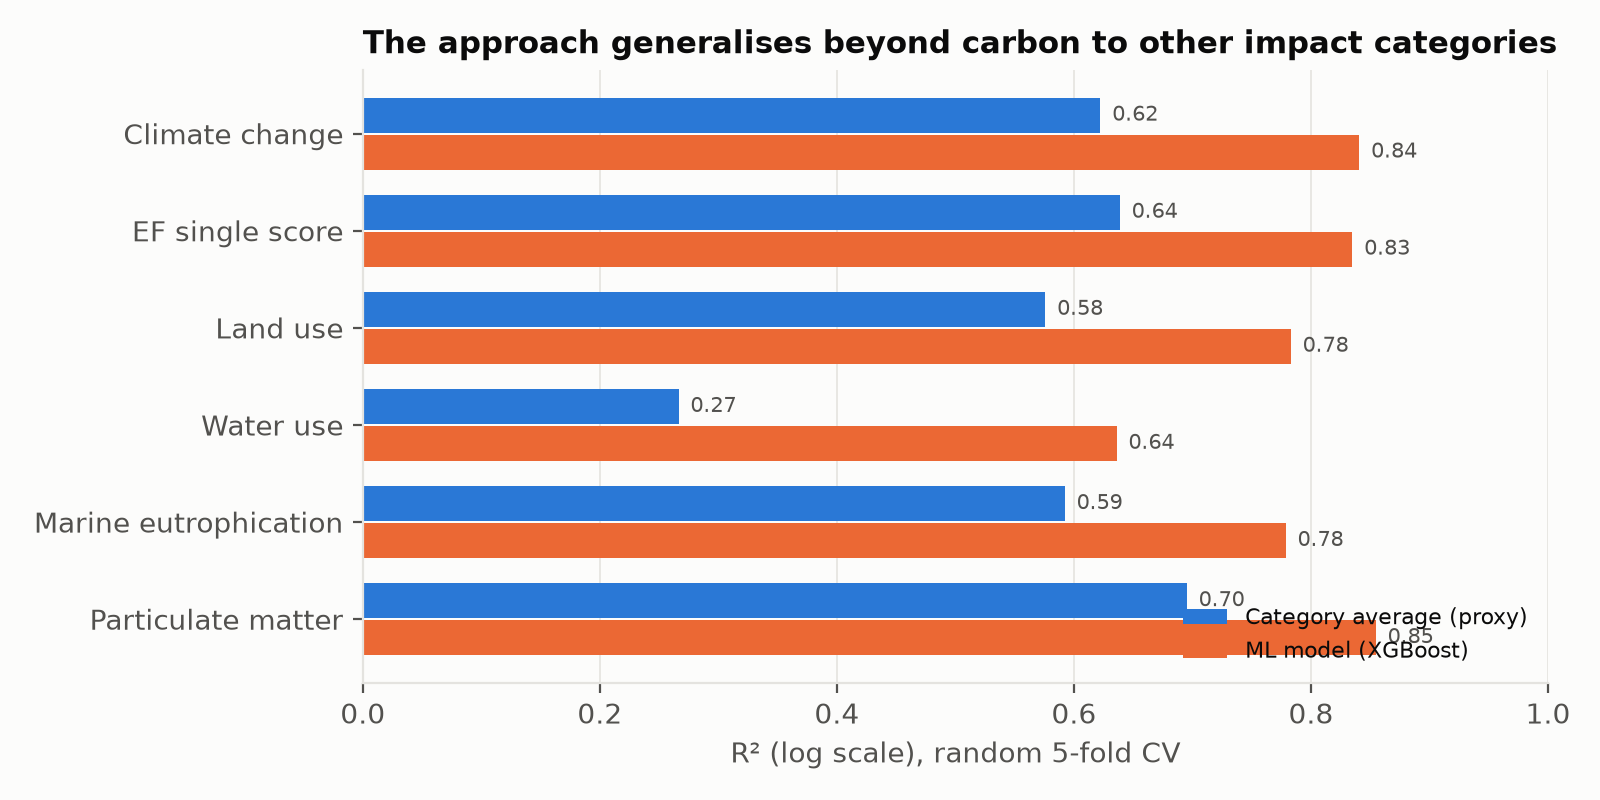
\includegraphics[width=0.85\textwidth]{f8_multi_impact}
\caption{The same pipeline, retrained per indicator, beats the proxy on all six impact categories.}
\label{fig:e3}
\end{figure}

The same pipeline, retrained per indicator without any change, improves on the proxy for every
category (Table~\ref{tab:e3}, Figure~\ref{fig:e3}). The largest relative gain is for \textbf{water
use} ($R^2$ 0.27 $\rightarrow$ 0.64): water scarcity depends strongly on crop and irrigation, which
category averages capture poorly but ingredient and name features capture well. Land use and
water remain the hardest indicators, consistent with their strong dependence on sourcing
location, which is not among the inputs.

\section{E4 -- Calibrated uncertainty}
\label{sec:e4}

\begin{table}[ht]
\centering\small
\caption{Mondrian conformal 90\% intervals (nested calibration).}
\label{tab:e4}
\begin{tabular}{@{}lcc@{}}
\toprule
Scheme & Empirical coverage & Median interval \\
\midrule
Random CV & 91.1\% & $\hat I\ \times\!/\!\div\ 2.0$ \\
Leave-sub-group-out CV & 87.2\% & $\hat I\ \times\!/\!\div\ 3.3$ \\
\bottomrule
\end{tabular}
\end{table}

\begin{figure}[ht]
\centering
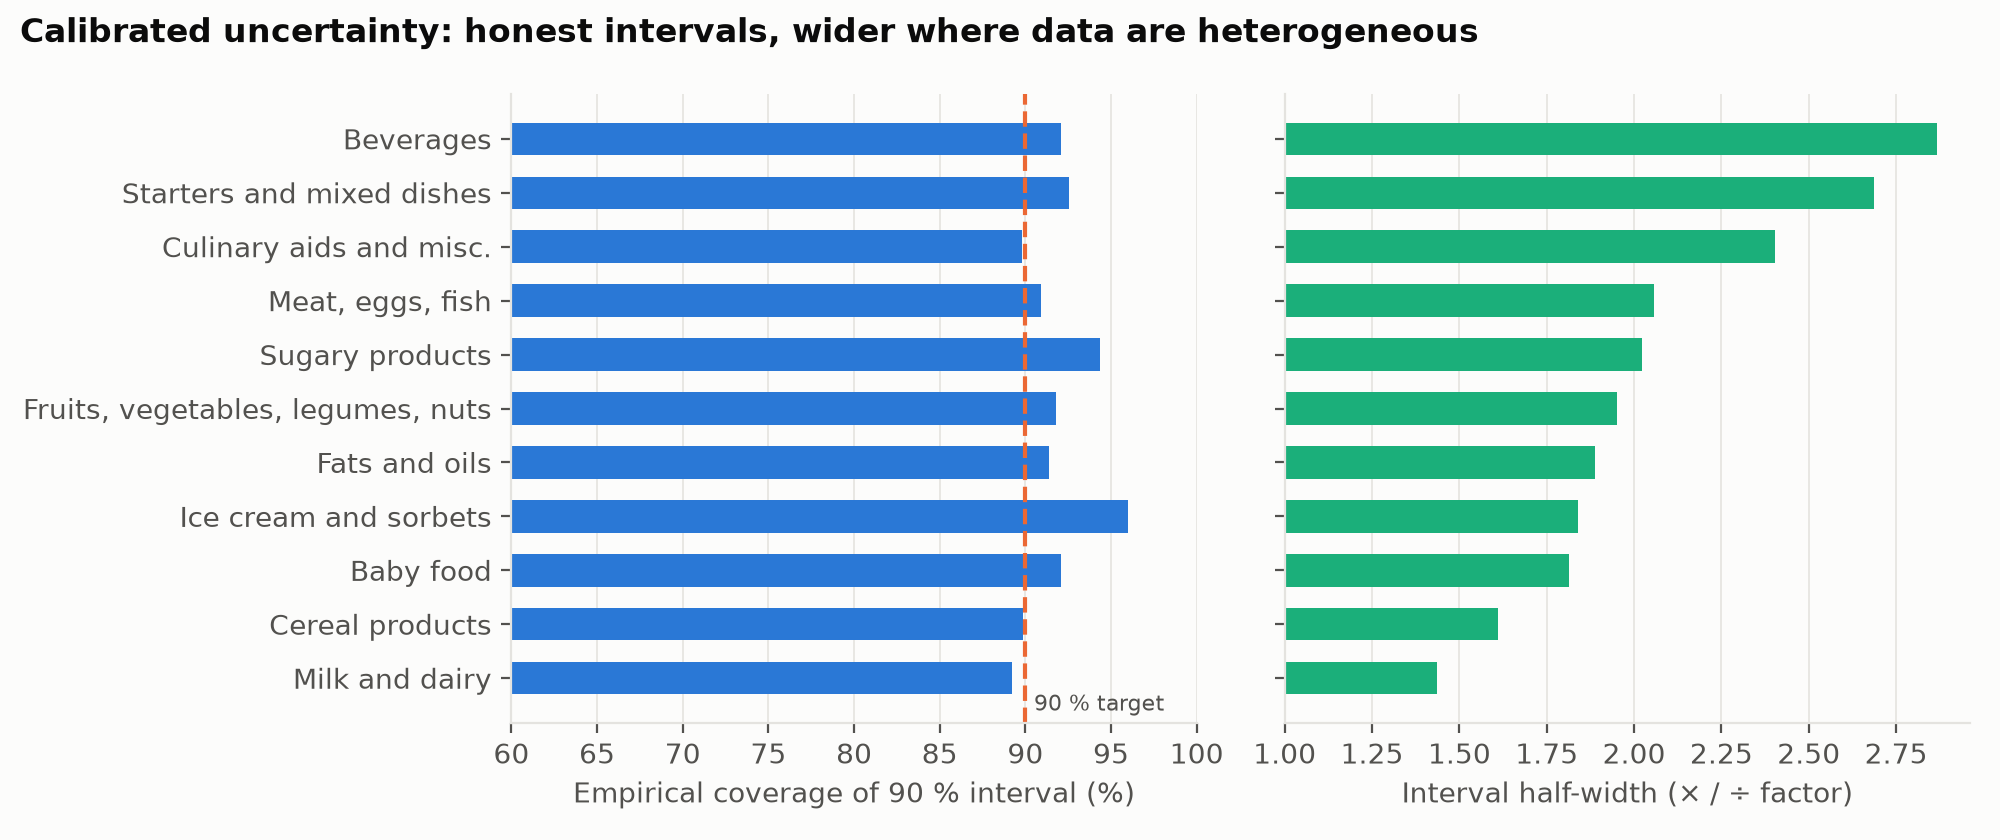
\includegraphics[width=\textwidth]{f10_conformal}
\caption{Per-group coverage (left) and interval half-width as a multiplicative factor (right), random CV.}
\label{fig:conformal}
\end{figure}

Under random CV the 90\% intervals achieve 91.1\% coverage, i.e.\ they are \emph{calibrated}
(Table~\ref{tab:e4}). Coverage is close to the target in every food group (89--96\%,
Figure~\ref{fig:conformal}), while widths adapt to difficulty: dairy products get
$\times\!/\!\div\,1.4$, mixed dishes $\times\!/\!\div\,2.7$ and beverages $\times\!/\!\div\,2.9$.
This is the practical value of the Mondrian variant.

On unseen sub-groups, overall coverage drops slightly to 87.2\% and intervals widen to
$\times\!/\!\div\,3.3$. The aggregate hides an instructive failure: coverage falls to 46\% for
\emph{milk and dairy}, 71\% for \emph{culinary aids} and 72\% for \emph{sugary products}. Dairy
sub-groups differ systematically (e.g.\ cheeses are several times more impactful than milks per
kg), and the calibration residuals, drawn from the remaining dairy sub-groups, are too small for
a new one. This is exactly the exchangeability assumption of conformal prediction being violated
under distribution shift, and it is reported here because it defines where the tool's intervals
should not be trusted: genuinely new product types within otherwise homogeneous groups.

\section{E5 -- Mapping descriptions to LCA datasets (Module B)}
\label{sec:e5}

\begin{table}[ht]
\centering\small
\caption{Mapping benchmark (2,451 queries per task). ``Borrow ${<}2\times$'': share of top-1 matches whose footprint is within a factor of two of the true product.}
\label{tab:e5}
\begin{tabular}{@{}lcccccc@{}}
\toprule
& \multicolumn{3}{c}{T1: French name $\rightarrow$ English DB} & \multicolumn{3}{c}{T2: 3-word query $\rightarrow$ full name} \\
\cmidrule(lr){2-4}\cmidrule(l){5-7}
Encoder & Top-1 & Top-5 & Borrow${<}2\times$ & Top-1 & Top-5 & Borrow${<}2\times$ \\
\midrule
TF-IDF char n-gram & 27.7 & 48.3 & 63.4 & 69.4 & 92.2 & 93.8 \\
MiniLM-L12 multilingual & 28.4 & 43.0 & 64.7 & 64.7 & 87.0 & 93.5 \\
LaBSE & \textbf{59.7} & \textbf{76.8} & \textbf{84.0} & 62.2 & 79.2 & 89.3 \\
E5-base multilingual & 48.2 & 67.5 & 78.3 & 74.0 & 94.6 & \textbf{97.1} \\
\textbf{E5-small (chosen)} & 47.1 & 66.0 & 78.8 & \textbf{75.0} & \textbf{94.9} & 96.8 \\
Hybrid TF-IDF + E5-small & 34.8 & 58.2 & 68.7 & 71.5 & 93.2 & 94.8 \\
\bottomrule
\end{tabular}
\end{table}

\begin{figure}[ht]
\centering
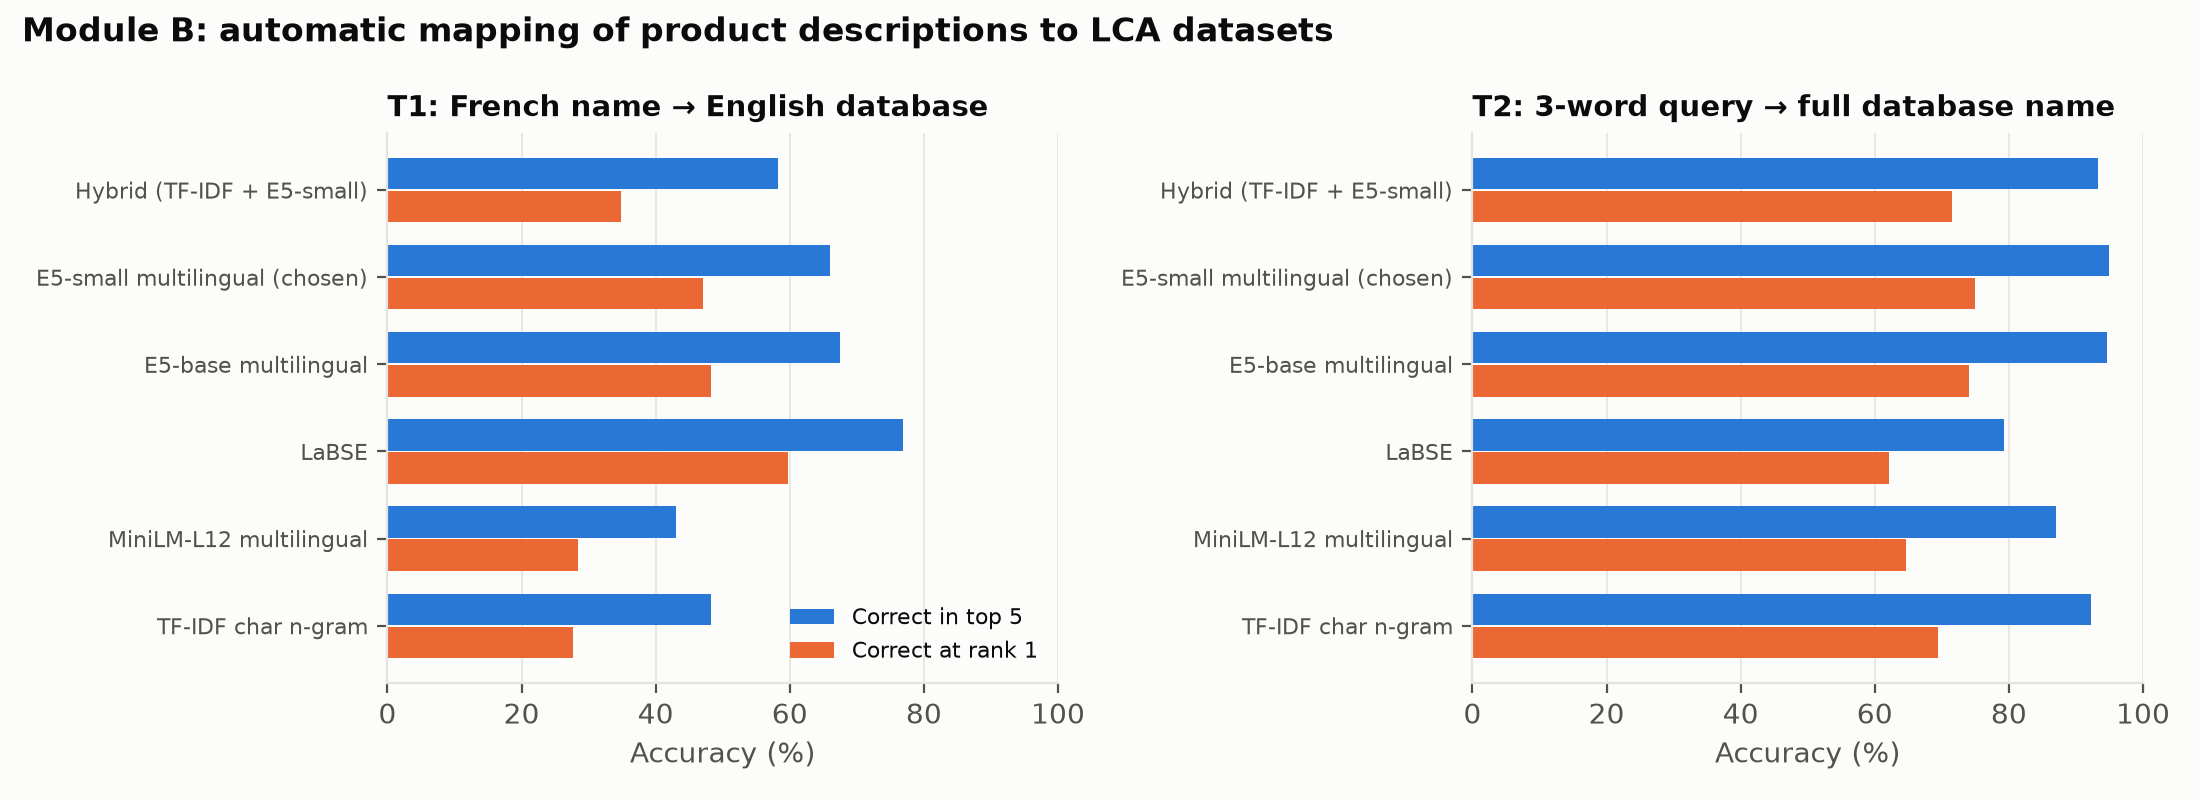
\includegraphics[width=\textwidth]{f9_matching}
\caption{Top-1 and top-5 mapping accuracy for both tasks.}
\label{fig:e5}
\end{figure}

Table~\ref{tab:e5} and Figure~\ref{fig:e5} answer \textbf{RQ4}. On the realistic terse-query task,
E5-small retrieves the exact dataset at rank 1 for 75\% of queries and within the top five for
95\%; borrowing the top-1 footprint lands within a factor of two of the truth for 97\% of queries.
Because the correctness criterion is strict (exact name), many ``errors'' are near-duplicates
(raw vs.\ cooked, fresh vs.\ frozen): 96\% of top-1 matches fall in the correct sub-group.

Three findings shaped the design:
\begin{itemize}
  \item \textbf{Encoder choice matters more than expected.} The widely used MiniLM model is no
  better than lexical TF-IDF across languages (28\% top-1), while E5 and LaBSE are far better.
  \item \textbf{No single best encoder.} LaBSE, trained for translation pairs, is best cross-lingually
  (60\% top-1) but worst on terse queries; E5-small is best on terse queries and second-best
  cross-lingually while being about four times smaller than E5-base. E5-small was chosen because
  terse queries are the primary use case.
  \item \textbf{Naive hybrids can hurt.} Averaging TF-IDF and E5 scores \emph{reduced} accuracy,
  because the two similarity scales have very different ranges; E5 alone is used.
\end{itemize}

\section{Explainability (SHAP)}
\label{sec:shap}

\begin{figure}[ht]
\centering
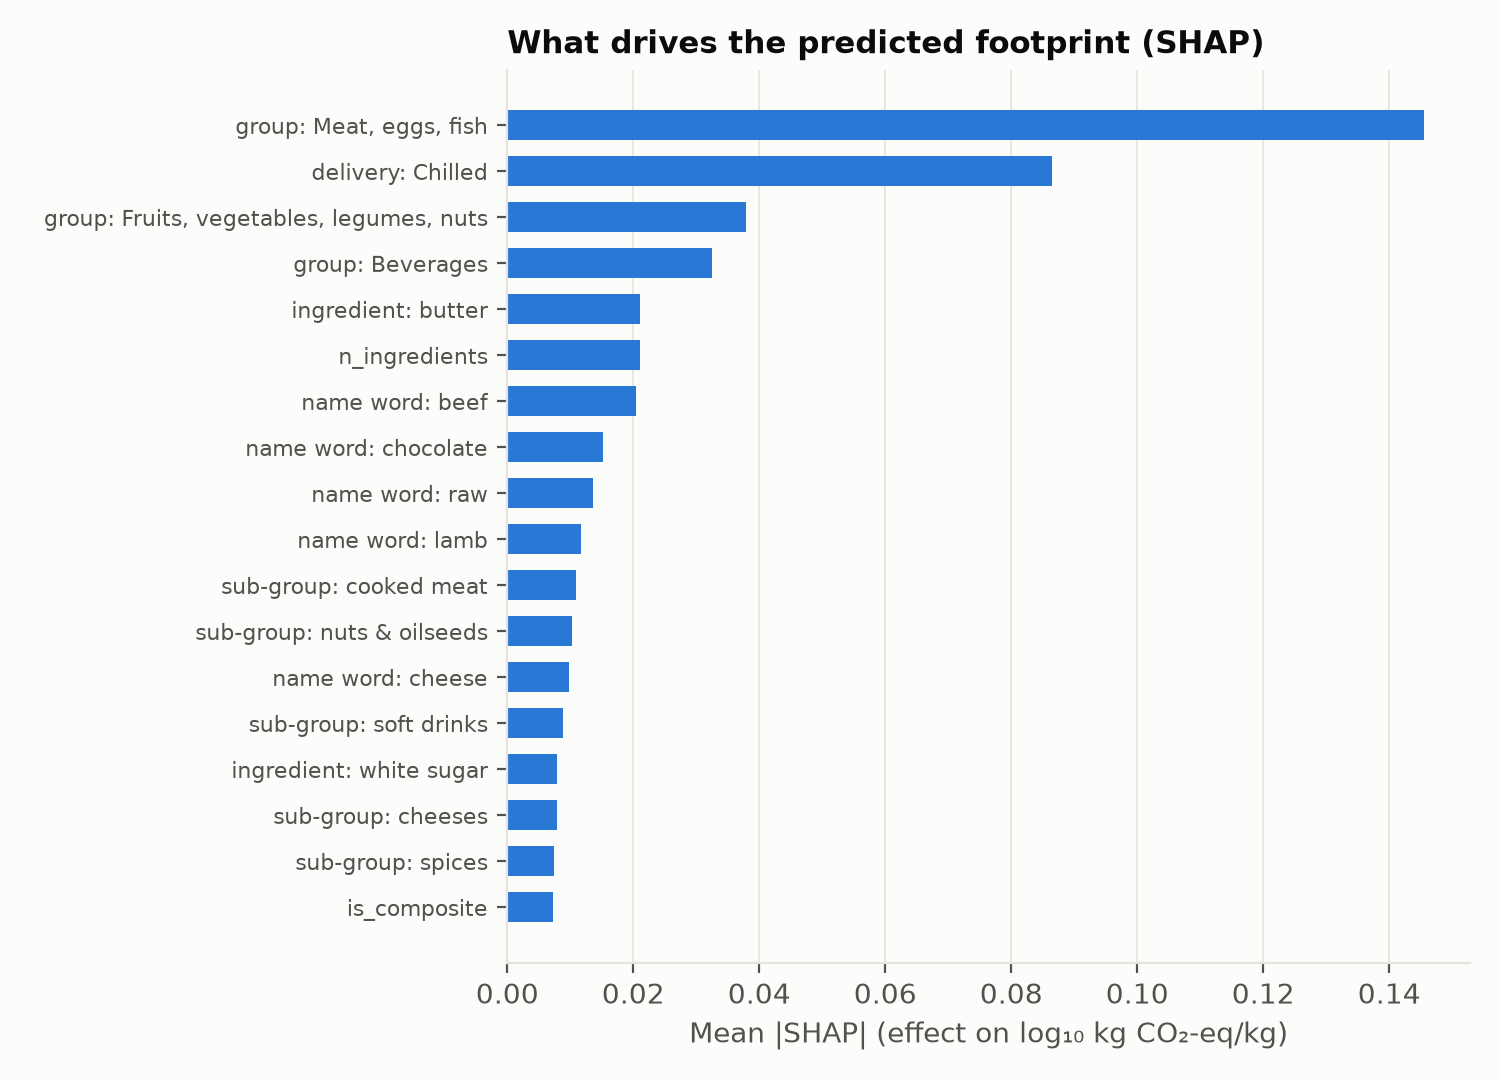
\includegraphics[width=0.85\textwidth]{f6_shap_importance}
\caption{Global feature importance: mean absolute SHAP value on the $\log_{10}$ scale.}
\label{fig:shap}
\end{figure}

\begin{figure}[ht]
\centering
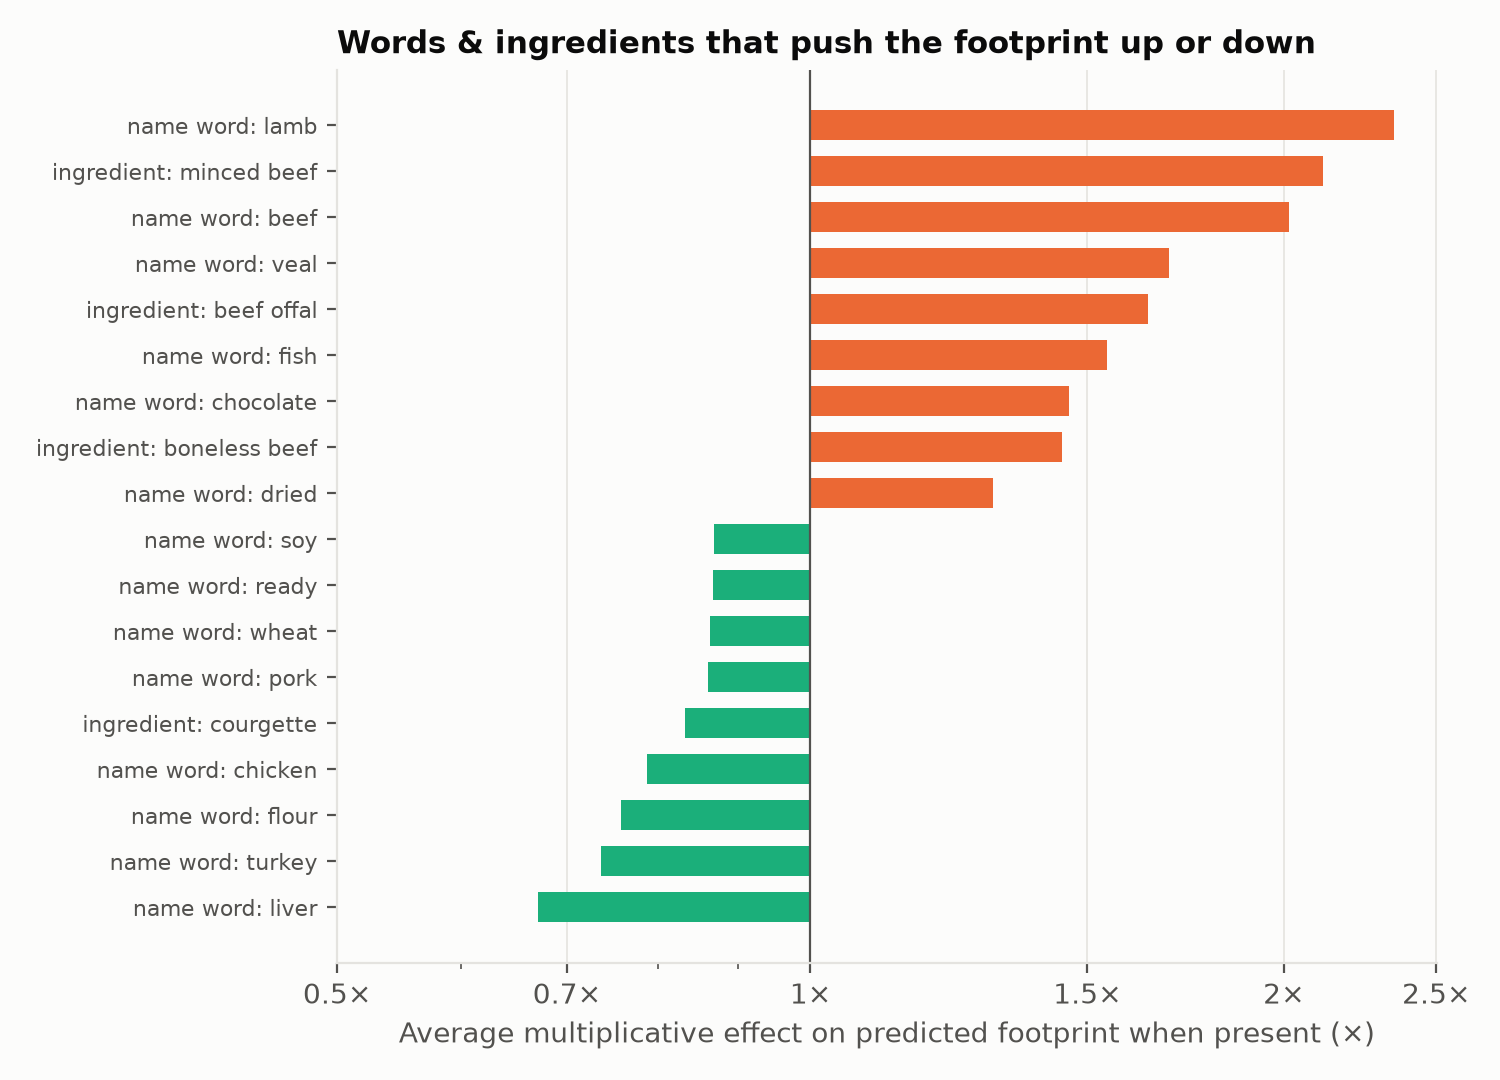
\includegraphics[width=0.85\textwidth]{f7_shap_direction}
\caption{Average multiplicative effect of name words and ingredients when present (orange: raises, green: lowers the estimate).}
\label{fig:shapdir}
\end{figure}

Figures~\ref{fig:shap} and~\ref{fig:shapdir} answer \textbf{RQ3}. Globally, the most influential
features are membership of the meat/eggs/fish group, chilled delivery, the fruit-and-vegetable and
beverage groups, butter as an ingredient, recipe size and the words \emph{beef}, \emph{chocolate}
and \emph{lamb}. Directionally (Figure~\ref{fig:shapdir}), \emph{lamb} multiplies the estimate by
about 2.4, minced beef by 2.1, \emph{beef} by 2.0 and \emph{veal} by 1.7, whereas \emph{chicken},
\emph{turkey} and \emph{pork} lower it relative to other meats. This ordering -- ruminant meat
$>$ pork $>$ poultry -- reproduces the well-established hierarchy in the food-LCA literature
\citep{poore2018}, and the large effect of \emph{chocolate} reflects the high land-use-change
emissions of cocoa. The model has therefore learned domain-consistent patterns rather than
spurious ones.

One important caveat for interpretation: \emph{chilled delivery} ranks second, but this does not
mean refrigeration causes high impacts. Chilled products are predominantly fresh meat, fish and
dairy, so ``chilled'' acts as a \emph{proxy} for animal products. SHAP explains the \emph{model},
not the physical system; causal statements require LCA modelling, not feature attributions.

\section{Summary of findings}

\begin{table}[ht]
\centering\small
\caption{Answers to the research questions.}
\begin{tabularx}{\textwidth}{@{}lX@{}}
\toprule
RQ & Finding \\
\midrule
RQ1 & XGBoost on pre-LCA features: $R^2_{\log}=0.84$, 91\% within $2\times$, Spearman 0.92 vs proxy 0.62 / 77\% / 0.82; consistent gains across six impact categories. \\
RQ2 & On unseen sub-groups $R^2_{\log}=0.62$ (proxy 0.33). 90\% conformal intervals are calibrated in-distribution (91.1\%) and slightly under-cover on new categories (87.2\%), with failures concentrated in dairy. \\
RQ3 & SHAP recovers the ruminant $>$ pork $>$ poultry hierarchy and the cocoa effect; ``chilled'' is a correlate of animal products, not a cause. \\
RQ4 & E5-small: 95\% top-5 on terse queries, 66\% top-5 cross-lingual; encoder choice is critical and no single encoder wins both tasks. \\
\bottomrule
\end{tabularx}
\end{table}

\chapter{Prototype Screening Tool}
\label{ch:tool}

The two modules are integrated into an interactive, multi-page web application built with
Streamlit (\texttt{app/}). It runs locally on a laptop CPU; after a one-time start-up of about
40--60 seconds (loading the language model), each query is answered in a few seconds. The
interface was designed for non-specialists: every number carries a plain-language explanation,
a tooltip and, where relevant, a warning. It has four pages:

\begin{description}
  \item[Estimate a product] free-text query $\rightarrow$ estimate, range, confidence and explanation;
  \item[Recipe \& portfolio] bill-of-materials screening with hotspot detection;
  \item[How the model thinks] global explanations and validation results;
  \item[About \& how to use] a four-step guide, a glossary (CO\textsubscript{2}-eq, range, SHAP,
  match) and the limitations.
\end{description}

\section{Single-product mode}

Figure~\ref{fig:app1} shows the main page for the query ``frozen breaded chicken nuggets''. One-click
example queries help first-time users, and the query is kept in the page URL so a result can be
shared. The page follows the framework of Figure~\ref{fig:arch}:

\begin{enumerate}
  \item \textbf{Result card (Module A).} The XGBoost estimate (4.8~kg~\co/kg) is shown with its
  Mondrian-conformal 90\% range (2.4--9.6) and the expert value of the closest database product
  (3.87), which lies inside the range. Two badges translate the numbers for a lay reader: an
  \emph{impact level} (low / below average / above average / high, from database quartiles) and a
  \emph{confidence} level that combines the match similarity with the width of the range. A
  percentile bar places the product among all foods and within its food group.
  \item \textbf{``Why this number?'' (explainability).} A generated sentence names the main drivers
  (``pushed up by \emph{Meat, eggs, fish} ×1.69 and \emph{Chilled} ×1.20; pulled down by
  \emph{chicken} ×0.79''). A \emph{waterfall chart} then starts from the typical food in the database
  (3.02~kg~\co/kg, the SHAP base value) and applies each feature's multiplicative SHAP effect in turn
  until the final estimate is reached, so the explanation adds up exactly to the prediction. A
  caption reminds the user that SHAP explains the model, not physical causation.
  \item \textbf{Closest products (Module B).} The five most similar AGRIBALYSE entries are listed
  with their footprints and a similarity bar.
  \item \textbf{Where the footprint comes from.} The expert life-cycle stage breakdown of the closest
  product (farming, processing, packaging, transport, shop, home) is shown for context; it is
  labelled as descriptive, because these values are never model inputs.
  \item \textbf{Lower-impact similar options.} Products from the same sub-group with a footprint at
  least 30\% lower are suggested, ranked by similarity to the matched product; for meat products,
  plant-based substitutes are added (here, soybean-based nuggets, $-63\%$). This turns the estimate
  into an actionable comparison.
  \item \textbf{Editable attributes.} Food group, sub-group, storage, preparation, packaging data
  source, air-freight flag and ingredients are pre-filled from the best match and can be edited in a
  collapsible panel; the estimate and explanation update immediately, which supports ``what-if''
  exploration.
\end{enumerate}

\begin{figure}[ht]
\centering
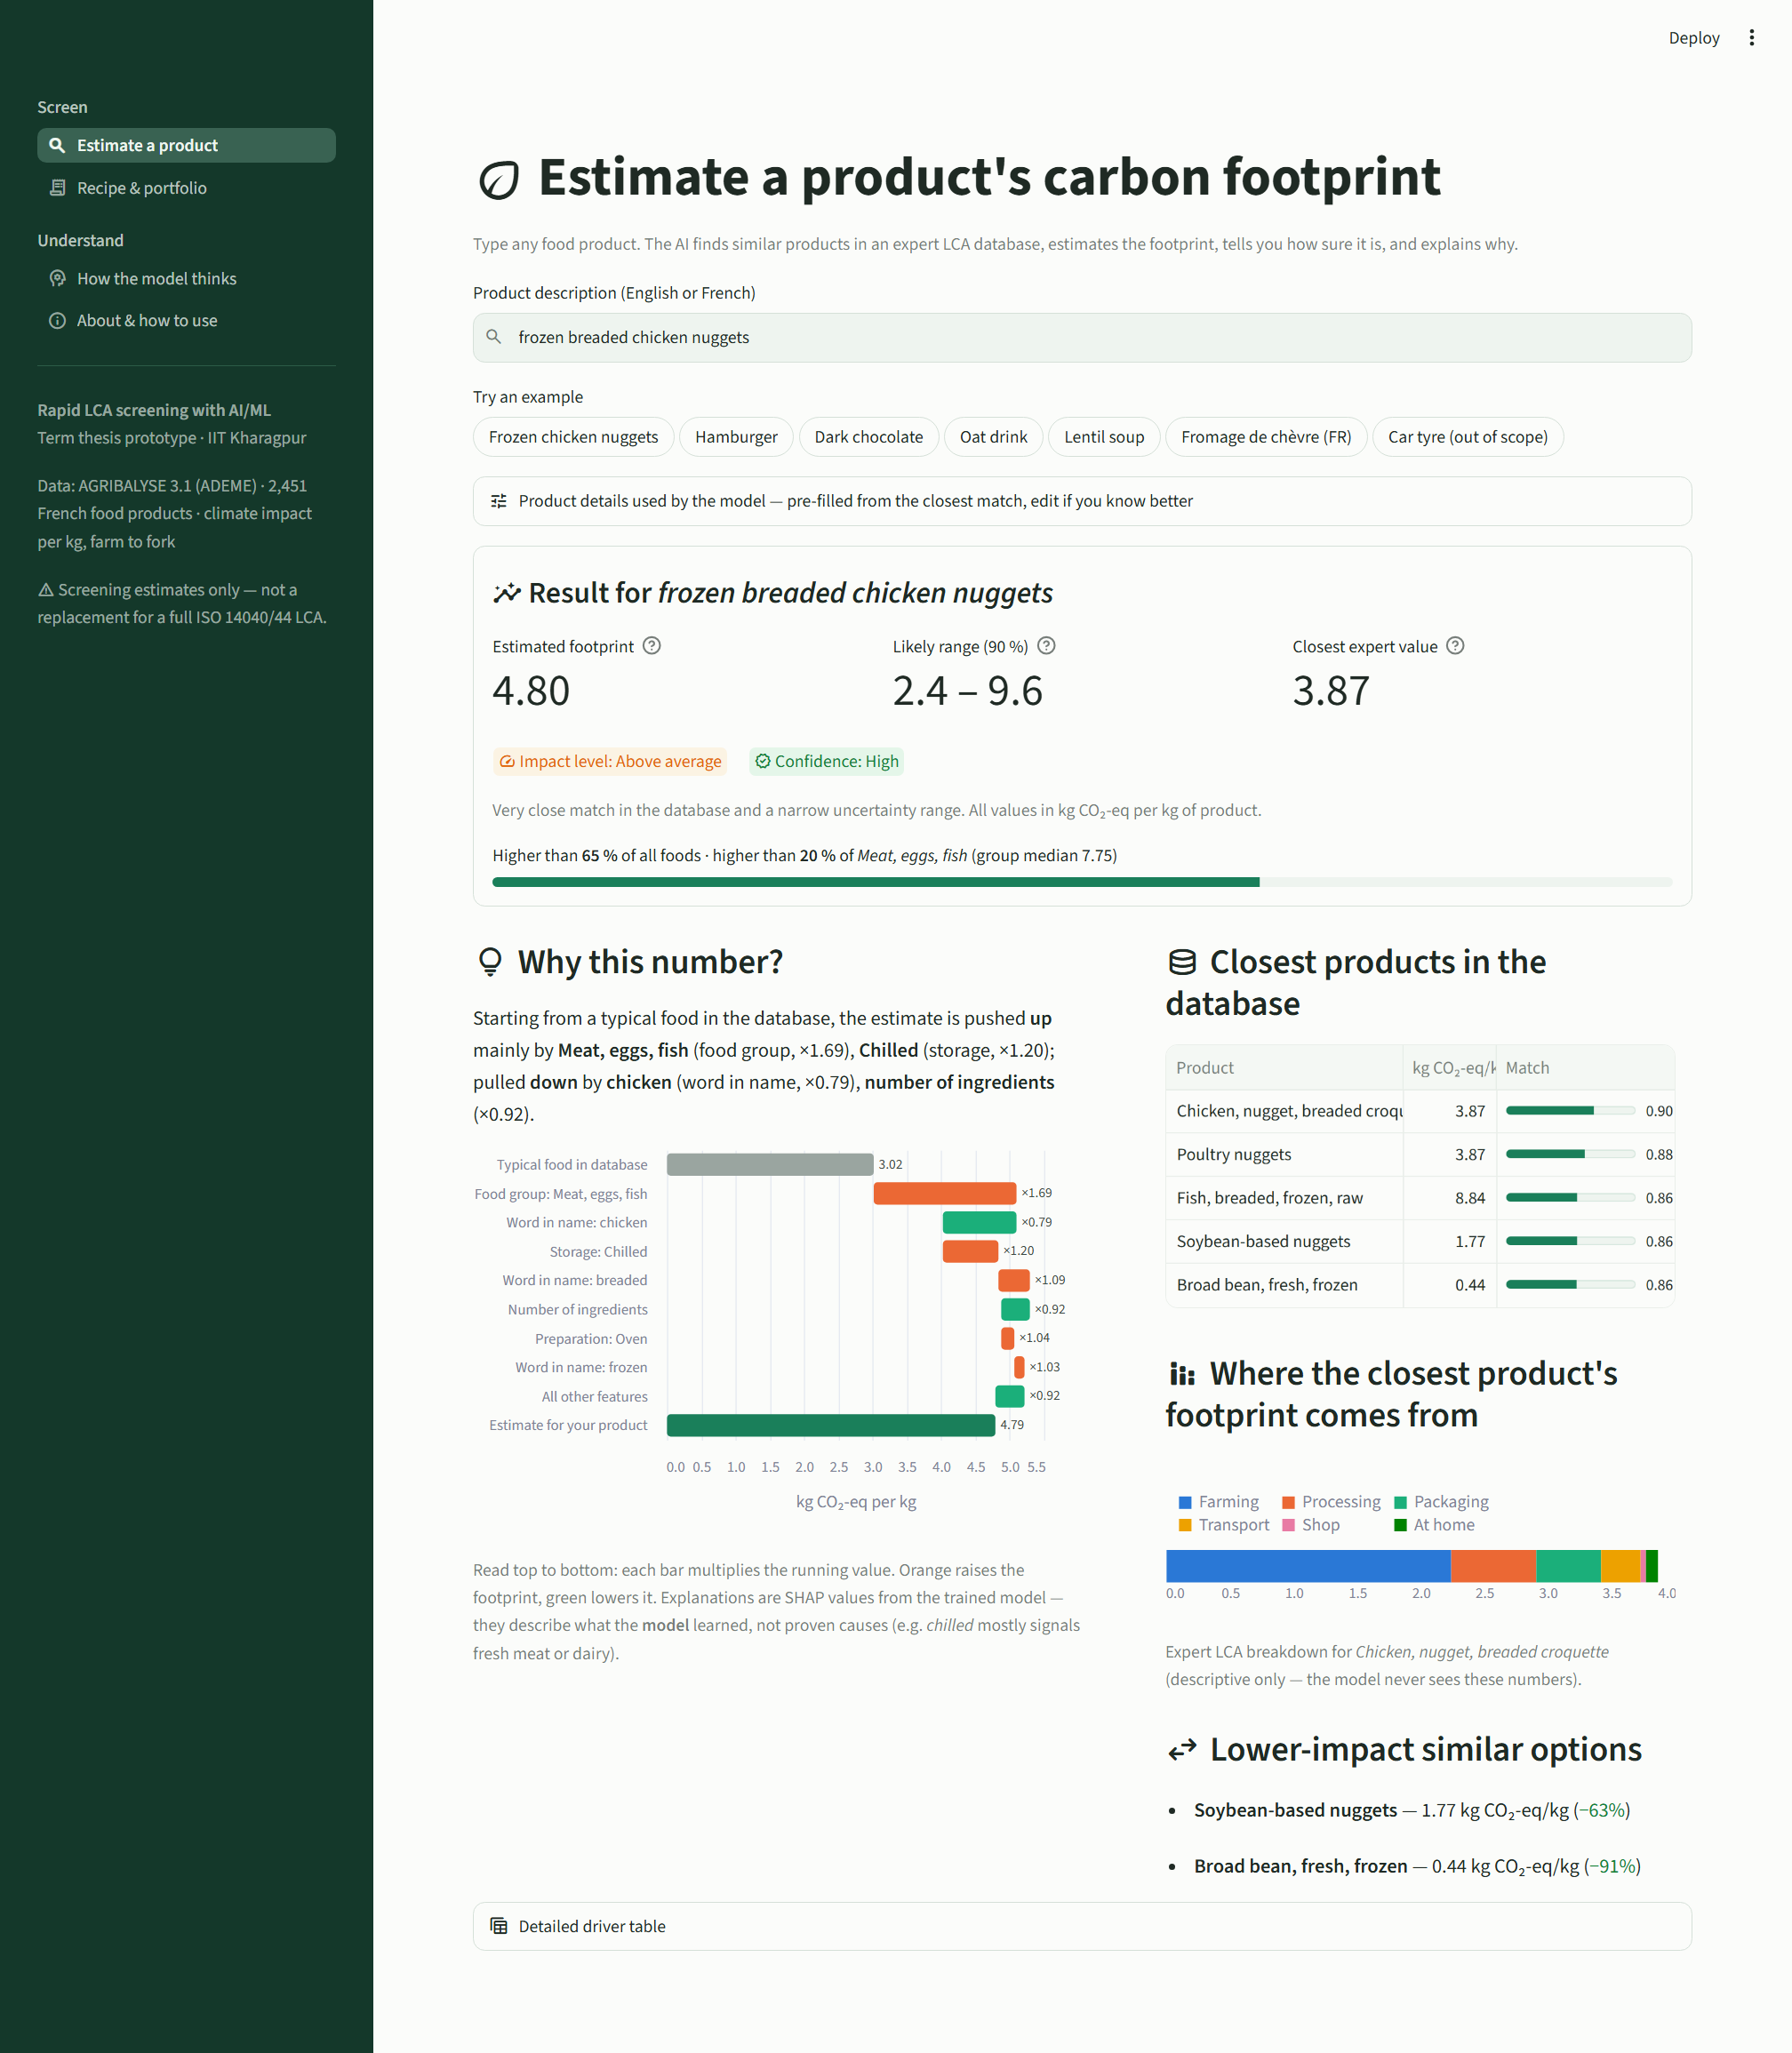
\includegraphics[width=\textwidth]{app_single}
\caption{Single-product screening for ``frozen breaded chicken nuggets'': result card with range, impact and confidence badges; waterfall explanation; closest datasets; stage breakdown of the closest product; and lower-impact alternatives.}
\label{fig:app1}
\end{figure}

\section{Applicability-domain warning}

For inputs outside the database's scope, nearest-neighbour retrieval still returns \emph{something};
without a guard, the user would receive a confident-looking but meaningless number. Figure~\ref{fig:app2}
shows the query ``car tyre'': the best similarity is 0.83, below the calibrated 0.85 threshold, so the
tool displays a prominent ``probably out of scope'' warning and the confidence badge drops to
\emph{Low}. This implements the recommendation of Song et al.\ \citep{song2017} that screening models
must state where they can be trusted.

The figure also shows \emph{why} the warning is essential. Behind it, the pipeline still produces
a plausible-looking number (6.0~kg~\co/kg, range 3.0--12.0), because the nearest dataset was a
pork product and the model faithfully estimates a pork product. The conformal interval cannot
detect this: it quantifies uncertainty \emph{within} the training distribution, not whether the
input belongs to it. Interval and applicability check are therefore complementary safeguards, and
neither can be dropped.

\begin{figure}[ht]
\centering
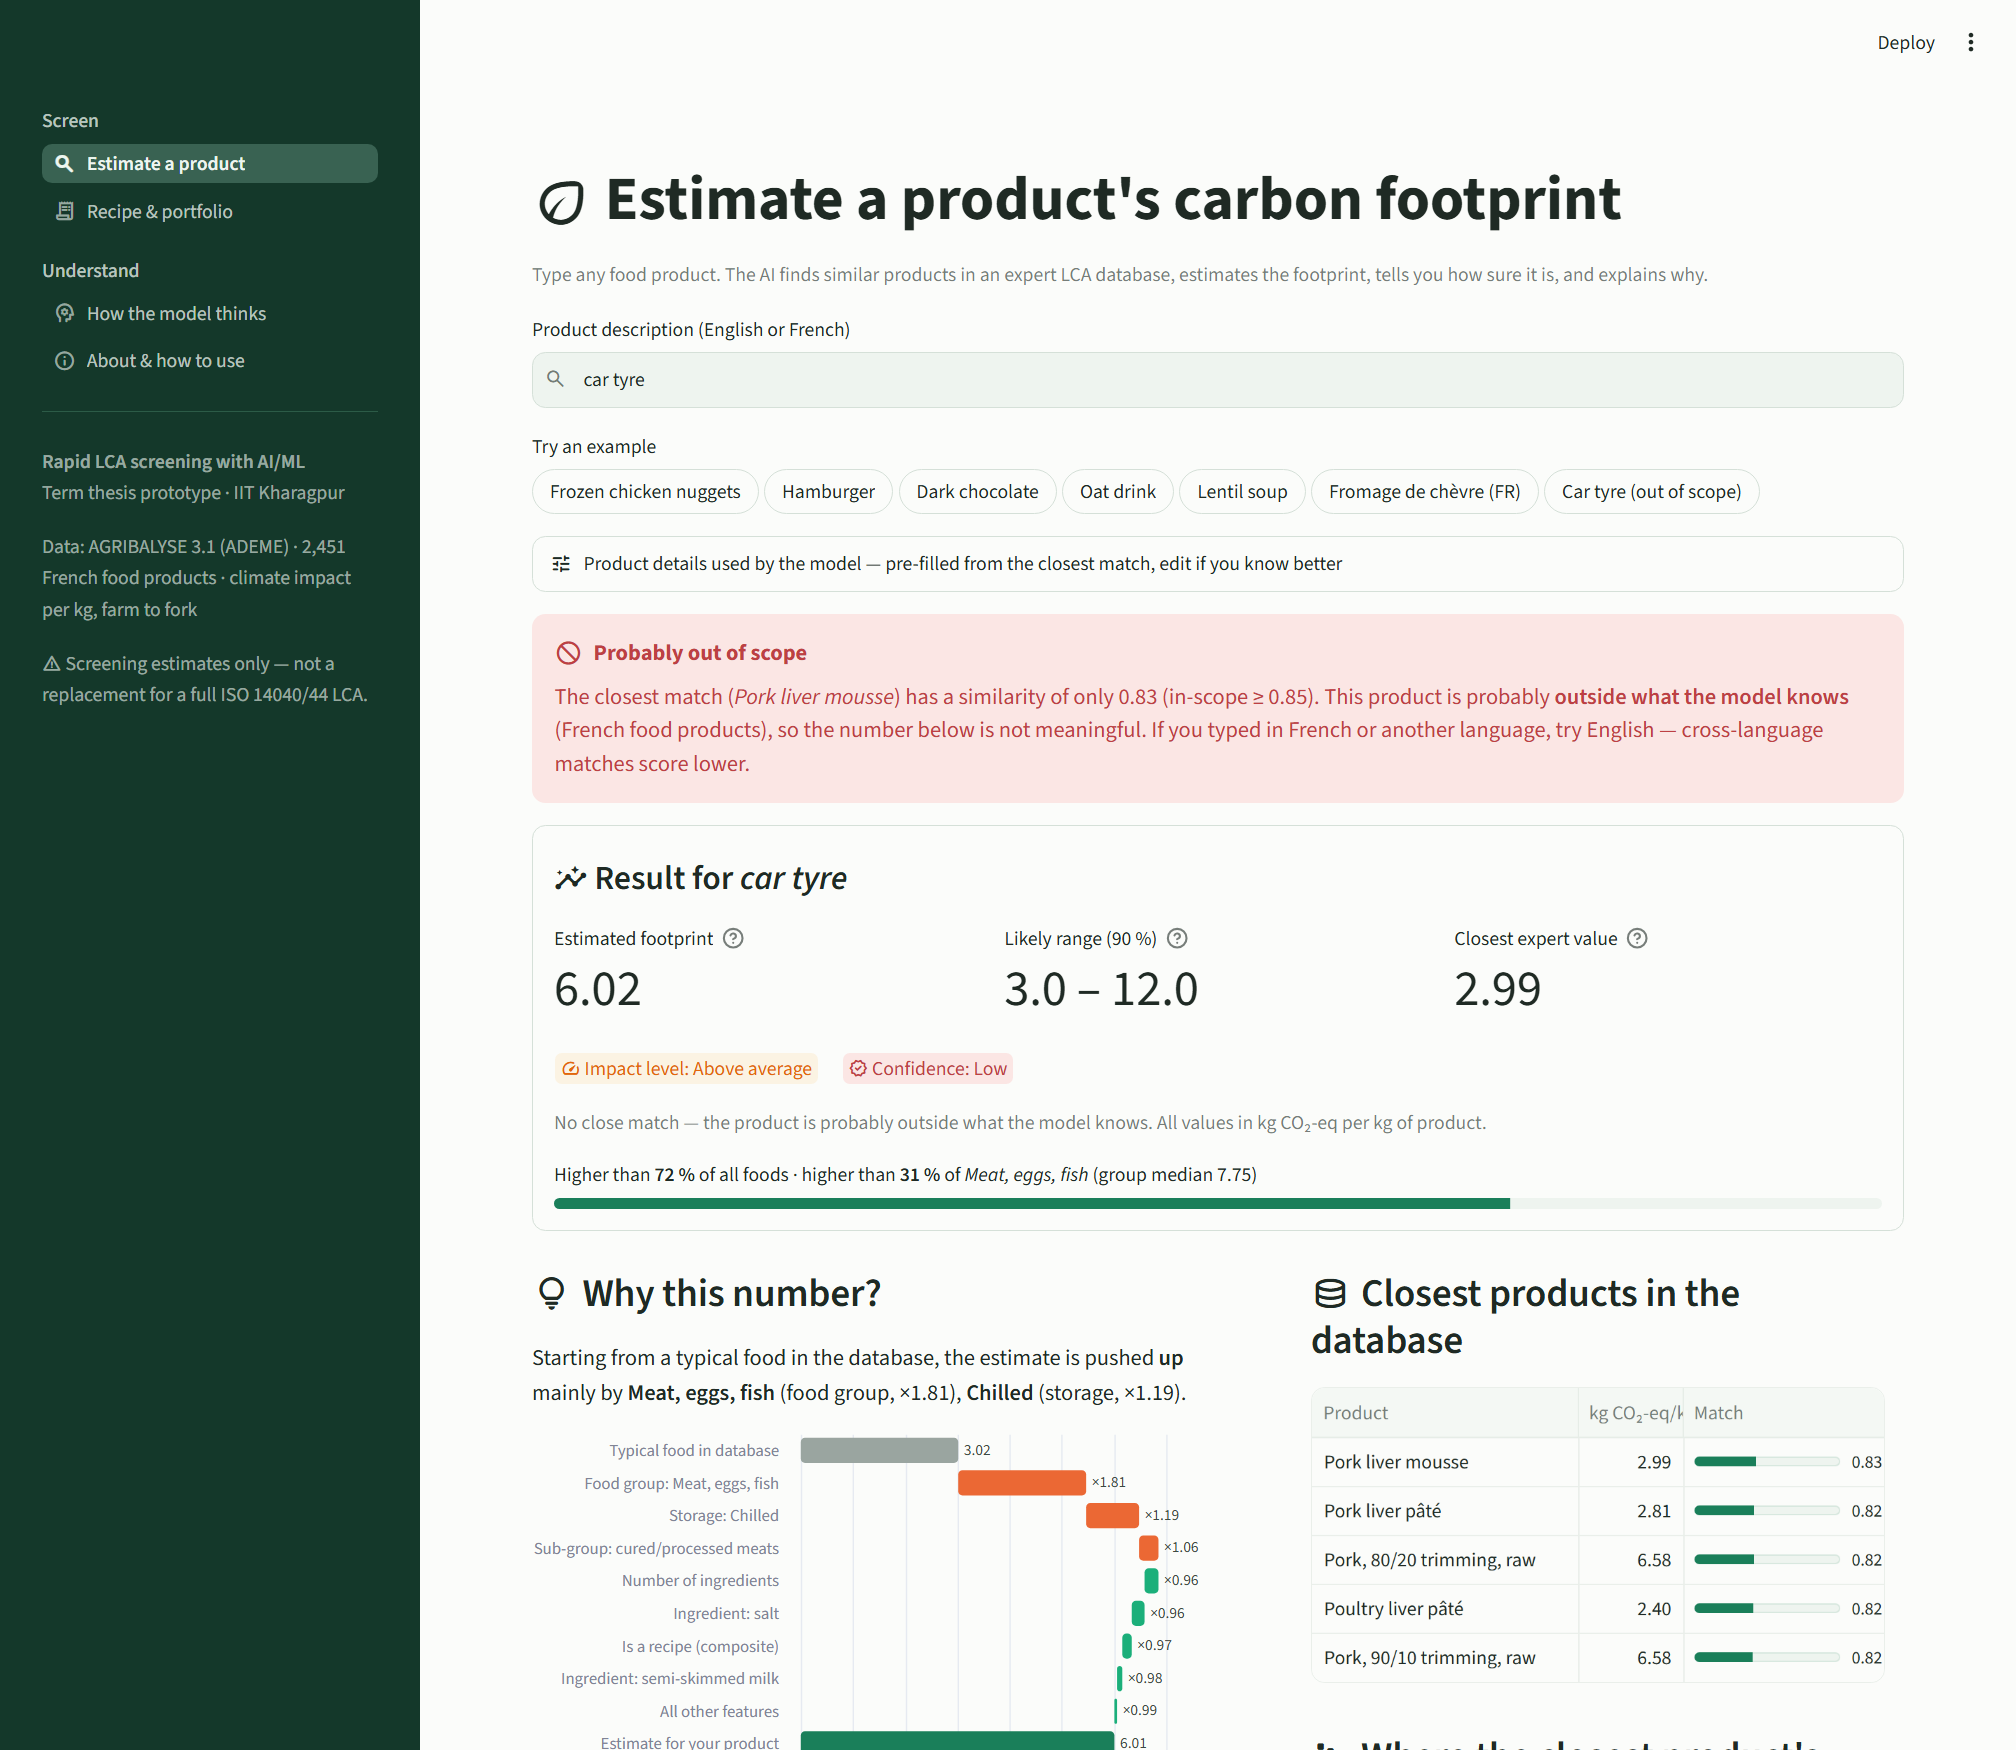
\includegraphics[width=0.9\textwidth, trim=0 0 0 0, clip]{app_ood}
\caption{Out-of-domain input (``car tyre''): low similarity triggers an explicit warning and a low-confidence badge.}
\label{fig:app2}
\end{figure}

\section{Recipe and portfolio mode}

The second page accepts an editable table of items and masses (e.g.\ 125~g minced beef, 150~g rice,
80~g tomato sauce, 30~g cheddar, 10~g olive oil). Each line is mapped, estimated and multiplied by
its mass. The page reports the total footprint, the biggest hotspot and its share, a ranked
contribution chart with the hotspot highlighted, per-item match quality, and lower-impact options
for the hotspot together with the saving each would bring to the recipe. In the example recipe,
minced beef contributes about 85\% of the total, and swapping it for soy-based mince would remove
most of the footprint. Low-similarity lines are flagged for manual review, results can be
downloaded as CSV, and item ranges are shown but not summed, because item errors are not
independent.

\section{Model insight page}

The ``How the model thinks'' page (Figure~\ref{fig:app3}) presents the global explanation and
validation evidence to users: headline metrics (91\% within a factor of two, $R^2=0.62$ on unseen
categories, 91\% interval coverage, 95\% top-5 matching), global SHAP importance, directional
effects of words and ingredients, an interactive comparison with the category-average shortcut
under both validation schemes, accuracy for six impact categories, and interval coverage by food
group, together with the honest caveat about new dairy sub-groups (Section~\ref{sec:e4}). This acts
as a built-in ``model card'', so users know the tool's intended use and failure modes.

\begin{figure}[ht]
\centering
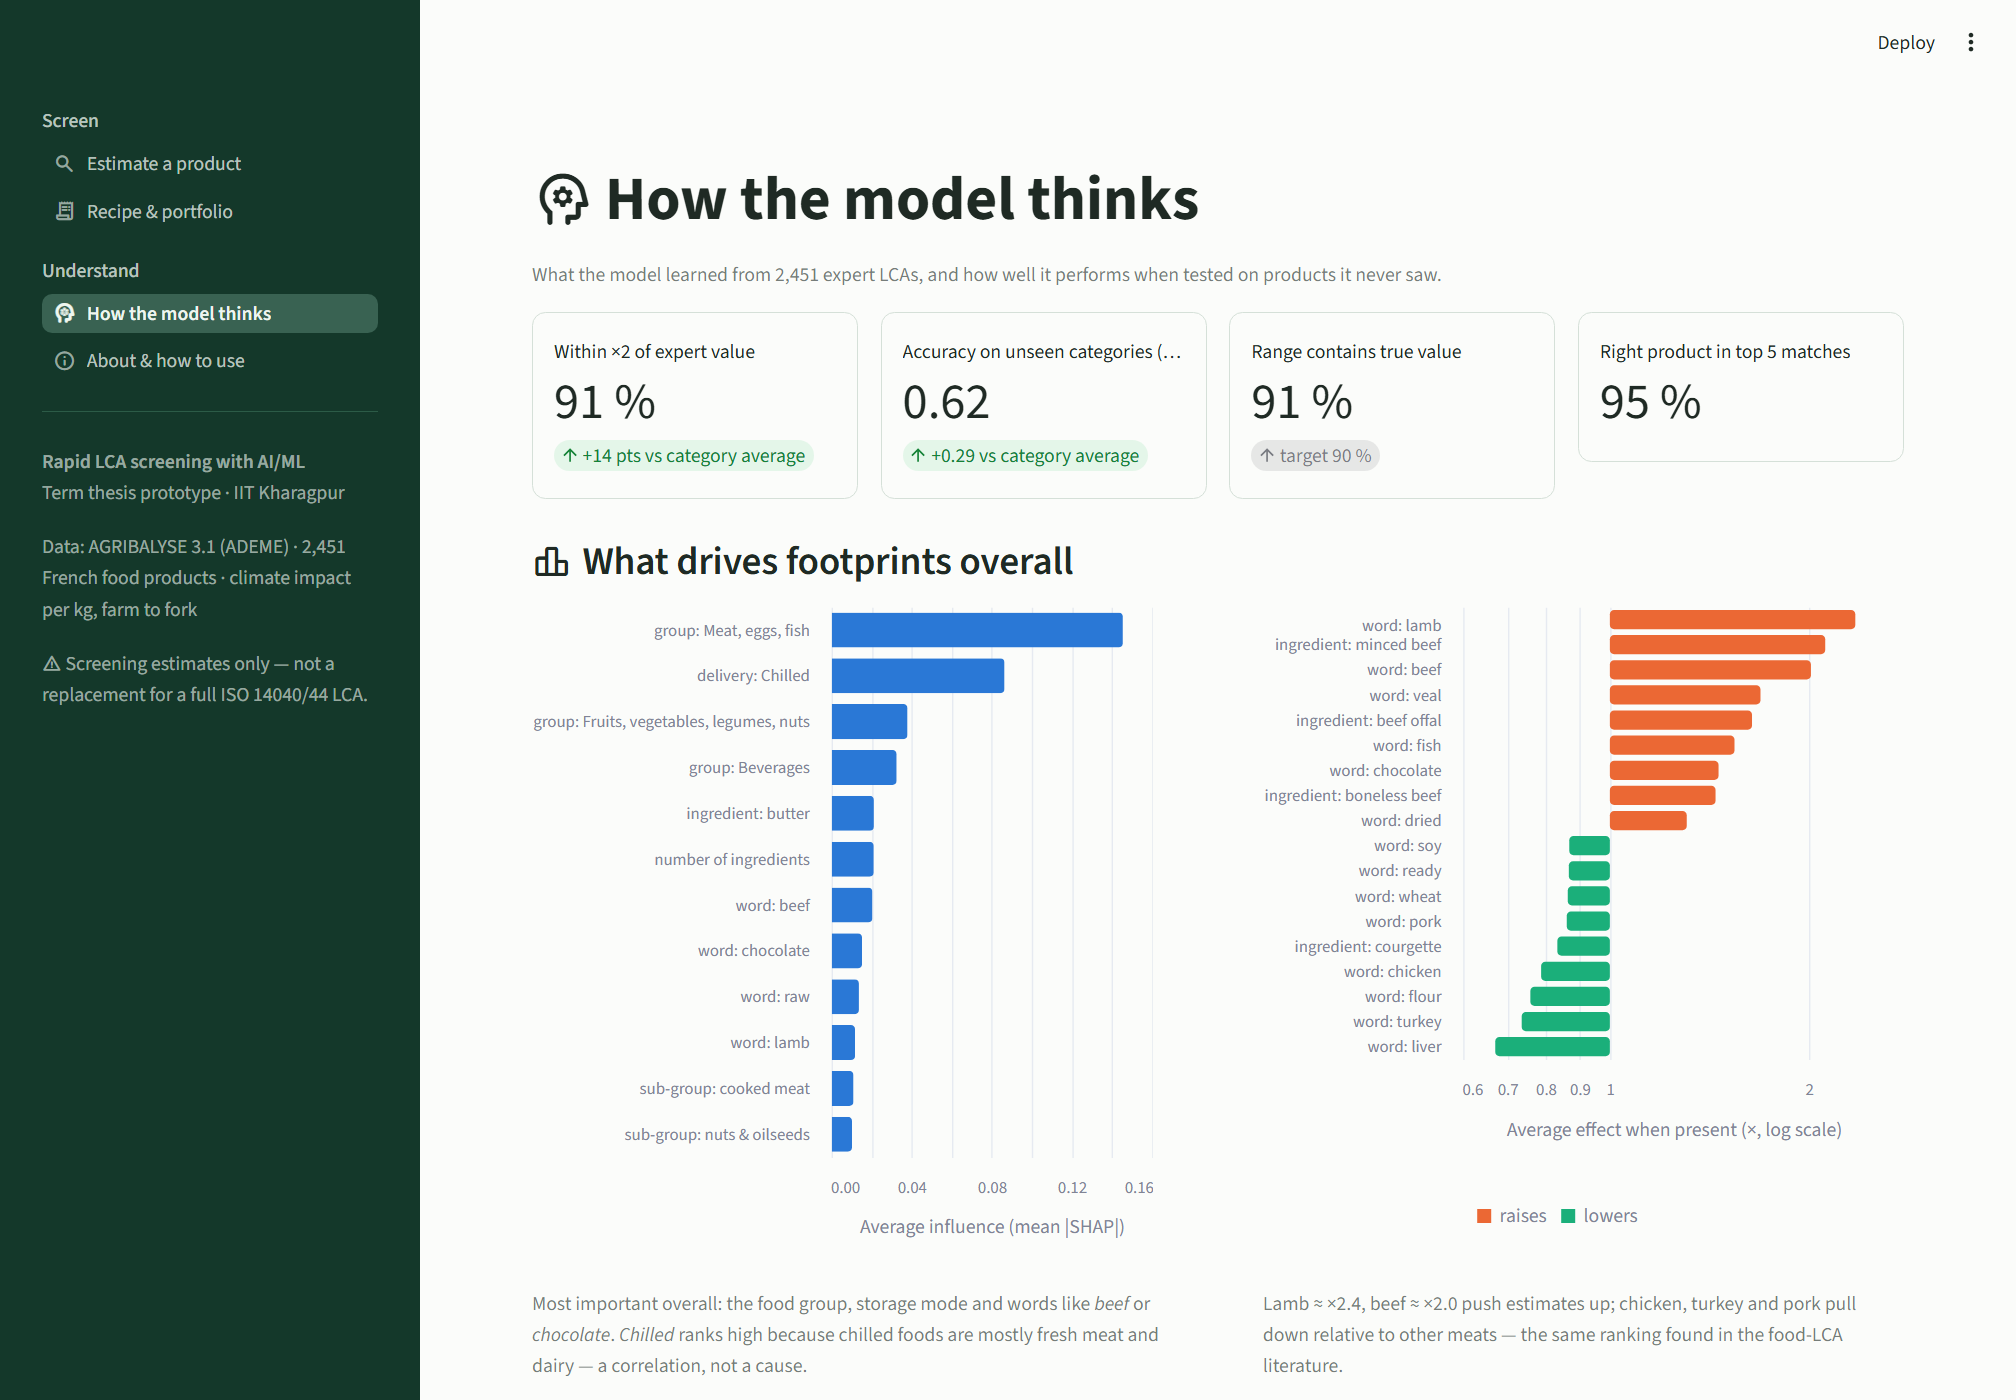
\includegraphics[width=\textwidth]{app_insights}
\caption{``How the model thinks'' page: headline validation metrics and global explanations.}
\label{fig:app3}
\end{figure}

\section{Intended use}

The tool is designed for \emph{screening}: prioritising which products, ingredients or suppliers
deserve a full LCA, comparing reformulation options early in design, and flagging likely hotspots
in large portfolios. It is \emph{not} intended to replace an ISO~14040/44 study, to produce EPDs,
or to support public comparative claims.

\chapter{Discussion}
\label{ch:discussion}

\section{What AI/ML adds to LCA -- and what it does not}

The results support a clear division of labour. ML does \emph{not} replace LCA: every target value
in this work was produced by a process-based LCA, and the model can only interpolate and moderately
extrapolate from that knowledge. What ML adds is \emph{speed and coverage at the screening stage}.
Once trained, the model estimates a new product in milliseconds from information a designer already
has, with an honest interval and an explanation. For portfolio-level decisions (which 50 of 2{,}000
products deserve a full LCA? which recipe reformulation is promising?), a Spearman rank correlation
of 0.92 and 91\% of estimates within a factor of two are far more useful than category averages,
and are available at essentially zero marginal cost.

The mapping module addresses a different, equally real cost: the analyst time spent translating
descriptions into database processes. A 95\% top-5 hit rate means that, in most cases, the analyst
only has to \emph{confirm} one of five suggestions rather than search a database -- the
human-in-the-loop design also recommended by CaML \citep{balaji2023caml}.

\section{Why the honest evaluation matters}

The gap between random CV ($R^2=0.84$) and leave-sub-group-out CV ($R^2=0.62$) is the central
methodological lesson. AGRIBALYSE contains families of near-identical products, so a random split
lets the model ``look up'' a sibling. Reporting only random-split accuracy, as is common, would
overstate how well an LCA surrogate works on genuinely new products by roughly a third of the
explained variance. The same lesson appears in uncertainty: conformal intervals calibrated
in-distribution under-cover on new dairy sub-groups (46\%). Distribution-free guarantees are only
as good as the exchangeability assumption behind them.

\section{Negative results}

Three design ideas that seemed promising did not work and were not adopted:
(i) stacking the embedding-kNN footprint as a feature (redundant with name words and harmful on new
categories); (ii) averaging lexical and semantic similarity scores (scale mismatch); and (iii) the
popular MiniLM multilingual encoder, which was no better than TF-IDF for cross-lingual mapping.
Reporting these protects future work from repeating them and shows that design choices were made on
evidence.

\section{Threats to validity}

\begin{description}
  \item[Internal validity] All vocabularies and calibration quantiles are fitted inside training
  folds; the kNN feature is computed leave-one-out; conformal coverage is assessed with nested CV.
  The only selection performed on reporting folds is a small $(k,T)$ grid for the non-adopted kNN
  variant. Hyper-parameters of XGBoost were fixed a priori; tuning would likely add a small
  improvement, so the reported accuracy is if anything conservative.
  \item[Construct validity] Targets are AGRIBALYSE values, which themselves carry uncertainty (mean
  DQR 2.46). The model learns AGRIBALYSE's modelling choices -- including its proxies -- not ``true''
  environmental impact. Agreement with AGRIBALYSE is the appropriate test for a screening surrogate
  of that database, but not evidence of physical accuracy.
  \item[External validity] All data describe the French food system (French agriculture, energy mix,
  logistics and consumption habits). Absolute numbers will not transfer directly to other countries.
  \item[Mapping benchmark] T1 and T2 are constructed from the database itself; real user queries
  may be noisier (typos, brand names, mixed languages).
\end{description}

\section{Limitations}

\begin{enumerate}
  \item \textbf{Rare but decisive attributes.} Air freight affects only two products in the data,
  so the model cannot learn its large effect (Section~\ref{sec:e1}). Any attribute that is rare in
  the training data but large in effect is a blind spot of purely data-driven models.
  \item \textbf{No ingredient masses.} AGRIBALYSE publishes which ingredients a recipe contains, not
  in what proportion. Mass shares would likely improve composite-food predictions considerably.
  \item \textbf{Origin and farming system.} Country of origin, organic vs.\ conventional and
  production system are not inputs, though they matter for land use and water.
  \item \textbf{Single domain.} Only food products are covered; extending to other sectors requires
  a comparable open product-level database.
  \item \textbf{Screening only.} Outputs are not suitable for ISO~14044 comparative assertions,
  EPDs or public claims.
\end{enumerate}

\section{Relevance for India}

India lacks a public, product-level food LCA database comparable to AGRIBALYSE, which is precisely
the situation in which screening tools are most useful and most dangerous. The framework transfers
in two ways. \emph{Methodologically}, the pipeline is database-agnostic: as Indian LCI datasets
become available, the same code can be retrained, and the leave-sub-group-out protocol and
applicability-domain check indicate how far the model can be trusted. \emph{Practically}, the
multilingual encoder already accepts descriptions in many languages, and the applicability check
correctly flags products absent from the French database (e.g.\ \emph{paneer}, similarity 0.84),
preventing silent misuse. A transfer-learning study -- training on AGRIBALYSE and recalibrating with
a small set of Indian LCAs -- is a natural next step.

\section{Implications}

\begin{itemize}
  \item \textbf{For practitioners:} use ML surrogates for prioritisation and hotspot screening, read
  the interval and the applicability flag, and confirm the mapping; reserve full LCA for decisions
  that need it.
  \item \textbf{For database providers:} publishing recipe proportions, origin and transport mode
  would directly improve the accuracy of data-driven screening.
  \item \textbf{For researchers:} report grouped (out-of-category) validation and calibrated
  uncertainty alongside random-split accuracy.
\end{itemize}

\chapter{Conclusions and Future Work}
\label{ch:conclusion}

\section{Conclusions}

This thesis set out to integrate AI/ML into Life Cycle Assessment in a way that is accurate,
honest about uncertainty, interpretable and usable. Using only the open AGRIBALYSE~3.1 database, it
built and evaluated a two-module framework and an interactive screening tool. The main conclusions
are:

\begin{enumerate}
  \item \textbf{ML substantially improves on category-average proxies.} From information available
  before an LCA, XGBoost predicts climate impact with $R^2_{\log}=0.84$, 91\% of products within a
  factor of two and a Spearman correlation of 0.92, versus 0.62, 77\% and 0.82 for the sub-group
  average. The improvement holds for all six impact categories tested.
  \item \textbf{Generalisation must be measured, not assumed.} On sub-groups never seen in training,
  accuracy falls to $R^2_{\log}=0.62$ -- still nearly double the proxy (0.33) -- showing that random
  splits overstate performance on genuinely new products.
  \item \textbf{Product identity is the key information.} Name words add more accuracy than any other
  feature block, consistent with the dominance of the agricultural stage.
  \item \textbf{Uncertainty can be reported rigorously.} Mondrian conformal intervals reach 91\%
  coverage at the 90\% target, with widths that adapt to each food group; their failure under
  distribution shift (new dairy sub-groups) is identified and documented.
  \item \textbf{Explanations agree with LCA knowledge.} SHAP recovers the ruminant $>$ pork $>$ poultry
  hierarchy and the cocoa effect, while highlighting that some important features (chilled storage)
  are correlates rather than causes.
  \item \textbf{Modern sentence embeddings make dataset mapping practical.} E5-small places the
  correct dataset in its top five for 95\% of terse queries; encoder choice matters greatly and no
  single encoder is best for both monolingual and cross-lingual mapping.
\end{enumerate}

\section{Future work}

\begin{enumerate}
  \item \textbf{Richer inputs:} recipe mass fractions, country of origin, transport mode and farming
  system, which would address the main failure modes found (air freight, tropical crops).
  \item \textbf{Hybrid physics--ML models:} compute a recipe-weighted sum of ingredient impacts and
  let ML learn only the residual (processing, packaging, losses), improving extrapolation.
  \item \textbf{Transfer to India:} recalibrate on a small set of Indian food LCAs and test whether
  conformal recalibration restores coverage.
  \item \textbf{Other sectors:} apply the framework to construction materials or chemicals where open
  product-level databases exist.
  \item \textbf{Large language models:} use LLMs to parse unstructured product sheets into the
  structured attributes the model needs, and to generate natural-language explanations from SHAP
  values -- with the conformal interval and applicability check retained as safeguards.
  \item \textbf{User study:} measure time saved and mapping accuracy with LCA practitioners using
  the tool on real bills of materials.
\end{enumerate}

\section{Closing remark}

AI/ML will not make Life Cycle Assessment unnecessary; it can make LCA thinking available
\emph{earlier} and \emph{at scale}. The guiding principle of this work -- predict only from what is
known before the LCA, measure generalisation honestly, attach calibrated uncertainty, explain every
estimate, and say clearly when the model is out of its depth -- is what makes such tools
trustworthy enough to use.


\renewcommand{\bibname}{References}
\bibliographystyle{unsrtnat}
\bibliography{refs}
\addcontentsline{toc}{chapter}{References}

\appendix
\chapter{Reproducibility}
\label{app:repro}

All code, data and results are in the project folder \texttt{BTP-2026/}:

\begin{tabular}{@{}ll@{}}
\texttt{data/raw/} & original AGRIBALYSE 3.1 CSV files \\
\texttt{data/processed/} & cleaned tables and cached embeddings \\
\texttt{src/prepare\_data.py} & cleaning, translation, no-leakage table construction \\
\texttt{src/embed.py} & E5-small embeddings of product names \\
\texttt{src/features.py} & feature builder (META, ING, TXT) and kNN predictor \\
\texttt{src/experiments.py} & E1--E4 and final model training \\
\texttt{src/matching\_eval.py} & E5 mapping benchmark \\
\texttt{src/ood\_threshold.py} & calibration of the out-of-scope similarity threshold \\
\texttt{src/figures.py} & all figures and SHAP analysis \\
\texttt{app/app.py} & Streamlit entry point (multi-page navigation) \\
\texttt{app/core.py} & shared logic: matching, estimation, explanations \\
\texttt{app/app\_pages/} & pages: estimate, recipe, insights, about \\
\texttt{results/} & all metric tables (CSV) and \texttt{RESULTS\_SUMMARY.md} \\
\end{tabular}

\medskip
\noindent Public repository: \url{https://github.com/krupalthakre/ai-lca-screening}.

\medskip
\noindent Commands (Python 3.12):
\begin{verbatim}
pip install -r requirements.txt
python src/prepare_data.py
python src/embed.py
python src/experiments.py
python src/matching_eval.py
python src/ood_threshold.py
python src/figures.py
streamlit run app/app.py
\end{verbatim}

\chapter{Model Settings}
\label{app:settings}

\begin{table}[ht]
\centering\small
\caption{Model hyper-parameters (fixed a priori; seed 42).}
\begin{tabular}{@{}ll@{}}
\toprule
Model & Settings \\
\midrule
Ridge & $\alpha=3.0$ \\
Random Forest & 500 trees, min\_samples\_leaf = 2, max\_features = 0.3 \\
XGBoost & 600 trees, learning rate 0.03, max depth 6, subsample 0.8, \\
        & colsample\_bytree 0.5, min\_child\_weight 2, $\lambda=1$ \\
kNN (E5) & $k=10$, softmax temperature $T=0.01$ (small grid: $k\in\{3,5,10\}$, $T\in\{0.005,0.01,0.02,1\}$) \\
Conformal & Mondrian by food group ($n_g\ge20$), $\alpha=0.10$, nested 5-fold calibration \\
Vocabularies & ingredients and name words with document frequency $\ge5$ in the training fold \\
\bottomrule
\end{tabular}
\end{table}

\noindent\textbf{Note on the kNN grid.} The $(k,T)$ grid was evaluated on the same cross-validation
folds used for reporting, which can make the kNN results slightly optimistic. This affects only the
kNN and stacked variants, which were \emph{not} adopted, so the conclusions are unaffected.


\end{document}
